% =============================================================================
% DRAFT (2026-11-10). To be rewritten by the author. [CHECK] marks a fact, a citation detail or a
% choice that must be confirmed; [TODO] marks missing content. Numbers in Section 7 come from
% experiments.py (results/summary.json); rerun it after any change to the setup.
% Build: latexmk -pdf paper.tex
% =============================================================================
\documentclass[11pt]{article}
\usepackage[margin=1in]{geometry}
\usepackage{amsmath,amssymb,amsthm,mathtools,bm}
\usepackage{booktabs}
\usepackage{graphicx}
\usepackage{xcolor}
\usepackage[hidelinks]{hyperref}
\usepackage[capitalize,noabbrev]{cleveref}

\newtheorem{theorem}{Theorem}[section]
\newtheorem{proposition}[theorem]{Proposition}
\newtheorem{lemma}[theorem]{Lemma}
\newtheorem{corollary}[theorem]{Corollary}
\newtheorem{assumption}[theorem]{Assumption}
\newtheorem{observation}[theorem]{Observation}
\theoremstyle{definition}
\newtheorem{definition}[theorem]{Definition}
\newtheorem{example}[theorem]{Example}
\theoremstyle{remark}
\newtheorem{remark}[theorem]{Remark}

\newcommand{\RR}{\mathbb R}
\newcommand{\CC}{\mathbb C}
\newcommand{\EE}{\mathbb E}
\newcommand{\inner}[2]{\langle #1,#2\rangle}
\newcommand{\norm}[1]{\lVert #1\rVert}
\newcommand{\tr}{\operatorname{tr}}
\newcommand{\range}{\operatorname{range}}
\newcommand{\nul}{\operatorname{null}}
\newcommand{\lmin}{\lambda_{\min}}
\newcommand{\lmax}{\lambda_{\max}}
\newcommand{\dsg}{\delta_{\mathrm{sg}}}
\newcommand{\Hb}{\bar H}
\newcommand{\xt}{x^\natural}
\newcommand{\T}{\mathcal T}
\newcommand{\chk}[1]{\textcolor{red!70!black}{[CHECK: #1]}}
\newcommand{\todo}[1]{\textcolor{blue!70!black}{[TODO: #1]}}

\title{Restricted contraction for preconditioned plug-and-play:\\
exact quasi-Newton spectra and compressed-sensing recovery with learned denoisers}
\author{Viktor Vigren\thanks{\chk{affiliation, WASP, funding acknowledgement, co-authors}}}
\date{Draft, \today}

\IfFileExists{results/numbers.tex}{% generated by make_numbers.py -- do not edit
\newcommand{\EXPdistinct}{489}
\newcommand{\EXPrealdim}{3912}
\newcommand{\EXPrank}{3500}
\newcommand{\EXPdsup}{0.9864}
\newcommand{\EXPdlo}{899}
\newcommand{\EXPdhi}{3548}
\newcommand{\EXPdstar}{780}
\newcommand{\EXPdzero}{737}
\newcommand{\EXPlimsup}{9.70}
\newcommand{\EXPfinal}{1.55}
\newcommand{\EXPlimsupfactor}{6.3}
\newcommand{\EXPepszero}{0.134}
\newcommand{\EXPostrowski}{0.9811}
\newcommand{\EXPobsrate}{0.9806}
\newcommand{\EXPiters}{4000}
\newcommand{\EXPboundviol}{0}
\newcommand{\EXPmincos}{0.140}
\newcommand{\EXPfired}{0}
\newcommand{\EXPapos}{0}
\newcommand{\EXPmaxlam}{117}
\newcommand{\EXPratio}{0.53}
\newcommand{\EXPzmfinal}{0.54}
\newcommand{\EXPthetaIlate}{1.55}
\newcommand{\EXPthetatable}{$2\cdot10^{-6}$ & 0.48 & 0\,\% & 25.3\\
$0.01$ & 0.48 & 0\,\% & 25.3\\
$0.1$ & 0.38 & 35\,\% & 14.5\\
$0.3$ & 0.81 & 77\,\% & 5.0\\
$0.6$ & 1.19 & 99\,\% & 2.0\\}
\newcommand{\EXPR}{16}
\newcommand{\EXPdG}{737}
\newcommand{\EXPpropGtable}{$I$ & 1.0000 & 0.9841 & 3.628 & 2.381 & 2.361 & 0.0207\\
circulant (density) & 1.1026 & 0.9849 & 5.748 & 3.664 & 3.642 & 0.0233\\
ZMSHR1 (frozen; MC dynamic) & 1.0014 & 0.9848 & 0.569 & 0.223 & 0.095 & 0.1374\\
tangent-restricted $P_T$ & 1.0000 & 0.0000 & 0.018 & -- & -- & --\\}
\newcommand{\EXPkcohrand}{4.8--6.0}
\newcommand{\EXPkcohhaar}{88--199}
\newcommand{\EXPconsrand}{13--14}
\newcommand{\EXPconshaar}{46--243}
\newcommand{\EXPdrand}{40, 80, 160, 320}
\newcommand{\EXPdhaar}{76, 121, 305}
}{}
\begin{document}
\maketitle

\begin{abstract}
Plug-and-play (PnP) reconstruction alternates a data-consistency step with a learned denoiser. For
preconditioned PnP in compressed-sensing MRI, the available convergence theory requires
$(1+\epsilon)\,\rho(I-\alpha PA^*A)<1$. We show that this condition cannot hold when $A$ has a nontrivial null
space, that it is not sufficient as stated when $PA^*A$ is not normal, and that the constant in the companion
stability bound for the zero-memory self-scaling symmetric rank-one (ZMSHR1) preconditioner is pessimistic by a
factor $\approx 1/(2\dsg)=5\cdot10^{7}$ for the published parameters, because the safeguard behind it can never
activate. These facts follow from an exact formula for the ZMSHR1 matrix: its eigenvalues are
$\rho_k(1\pm\sin\vartheta_k)$, with $\rho_k$ the Barzilai--Borwein step and $\vartheta_k$ the secant angle.
We then replace global contraction by \emph{restricted} contraction. If the denoiser's secant acts on the error
as a nonexpansive map supported on a $d$-dimensional tangent space, up to a leakage $\eta$, then PnP approaches
the truth at a linear rate whenever a pairwise restricted constant $\delta$ of the data step satisfies
$\eta m(1-\delta+m)<1-\delta$, where $m$ bounds the data step. The error bound is explicit in noise, model mismatch
and leakage, and holds for undersampled operators and dynamic preconditioners, without a fixed-point
assumption. For random block sampling (non-Cartesian, multi-coil), a matrix Chernoff bound yields the
restricted condition with high probability once the number of shots exceeds a multiple of
$(\Phi_0/\lambda_-)\log(d/p)$: the sample complexity is proportional to the denoiser's tangent dimension, scaled
by a block coherence. Finally, preconditioning changes the PnP \emph{estimator}, not only the convergence path.
Locally, the noise part of the PnP limit is the best linear unbiased estimator on the tangent space if and only if
$P$ maps no data-visible direction orthogonal to the tangent space into it. The model mismatch inside the tangent
space, however, is amplified by $(\alpha\Pi_0PH\Pi_0)^{-1}$, which is up to the restricted condition number for
$P=I$. Density-compensation-type preconditioners fail on both counts. A tangent-restricted preconditioner attains
both the optimal variance and the unamplified bias. Toy experiments in which every hypothesis can be computed
illustrate each result. \chk{abstract length for the target journal}
\end{abstract}

\section{Introduction}\label{sec:intro}

Let $A:\RR^n\to\RR^q$ be a linear measurement operator, $y=A\xt+n$ the data, $f(x)=\tfrac12\norm{Ax-y}^2$ and
$H=A^*A$. Plug-and-play (PnP) methods \cite{venkatakrishnan2013,kamilov2023pnp} replace the proximal step of a
splitting method by a denoiser $D$. The simplest instance, PnP-ISTA, and its preconditioned variant P$^2$nP
\cite{hong2024p2np} read
\begin{equation}\label{eq:pnp}
  x_{k+1}=D\big(z_k\big),\qquad z_k=x_k-\alpha P_k\nabla f(x_k)=x_k-\alpha P_kA^*(Ax_k-y),
\end{equation}
with $P_k\succ0$ fixed or updated from iterate differences. In MRI, $A$ is a multi-coil, often non-Cartesian
Fourier operator. Without density compensation, $H$ is very ill-conditioned (the centre of $k$-space is
sampled far more densely than the periphery), and a preconditioner can reduce the iteration count by an order of
magnitude \cite{hong2024p2np}.

The convergence theory of \cite{hong2024p2np} follows the template of \cite{ryu2019}: the denoiser is
$(1+\epsilon)$-Lipschitz, the data step $I-\alpha PH$ is a contraction, and the product contracts if
$(1+\epsilon)\rho(I-\alpha PH)<1$. For a dynamic quasi-Newton preconditioner (ZMSHR1, built on
\cite{osborne1999,becker2012qn,becker2019qn,hong2024complexqn}) a stability bound is given whose constant depends
on the safeguard parameter as $1/\dsg$. The authors note that their bound becomes very large for the parameters
that work well, and that ``further analysis could lead to tighter results'' \cite[Sec.~III]{hong2024p2np}.

This paper supplies that analysis and goes further. Its starting point is that, in compressed sensing,
contraction can only come from the \emph{product} of denoiser and data step. The denoiser must remove exactly the
directions that the data cannot see. Any argument that bounds the two factors separately is therefore vacuous
when $A$ has a null space. The right objects are the denoiser's (secant) Jacobian, which for trained denoisers is
close to a projector onto a low-dimensional, signal-adaptive subspace \cite{mohan2020,kadkhodaie2021,kadkhodaie2024},
and the data step \emph{restricted} to such subspaces.

\paragraph{Contributions.}
\begin{enumerate}
\item \textbf{The existing conditions} (\cref{sec:setting}). The condition $(1+\epsilon)\rho(I-\alpha PH)<1$ is
  unsatisfiable when $\nul A\neq\{0\}$ (\cref{obs:vacuous}). It is also not sufficient when $PH$ is not normal: we
  give a two-dimensional counterexample with a $1$-Lipschitz denoiser and divergent iterates
  (\cref{prop:counterexample}). The operator norm restores the statement.
\item \textbf{Exact ZMSHR1 spectrum} (\cref{sec:zmshr1}). The ZMSHR1 matrix has eigenvalues
  $\rho(1-\sin\vartheta)$ (multiplicity $n-1$) and $\rho(1+\sin\vartheta)$ (\cref{lem:spectrum}). It follows that
  the safeguard of \cite{hong2024p2np} is inert unless $\dsg\geq\tfrac12\sqrt{\theta_1/\theta_2}$
  (\cref{cor:inert}), that $P_k\preceq\frac{1+\sqrt{1-\theta_1/\theta_2}}{\theta_1}I$ with no dependence on
  $\dsg$, and that the stability constant improves by a factor $\approx1/(2\dsg)$ (\cref{thm:stability}).
\item \textbf{Restricted contraction} (\cref{sec:restricted}). Under a secant tangent-structure assumption with
  leakage $\eta$ (\cref{ass:secant}), PnP with arbitrary (dynamic) preconditioners satisfies a coupled
  two-term recursion for the error to the \emph{truth}. It converges linearly to an explicit ball when
  $\eta m(1-\delta+m)<1-\delta$ (\cref{thm:restricted}). Soft thresholding satisfies the assumption with
  $\eta=0$ globally (\cref{ex:soft}). The exact local rate is
  $\rho\big(J_D(z_*)(I-\alpha PH)\big)$ (\cref{prop:local}).
\item \textbf{Sampling theorems} (\cref{sec:sampling}). For i.i.d.\ block sampling, the restricted constant is
  controlled with high probability once the number of shots is at least
  $\frac{3\Phi_0}{t^2\lambda_-}\log\frac{2d}{p}$. Here $\Phi_0$ is a block coherence of the tangent space at the
  truth and $\lambda_-$ the restricted expected curvature (\cref{thm:local}). A uniform version over a family of
  tangent spaces (\cref{thm:uniform}) addresses the ``moving sparsifying basis'' of a learned prior.
\item \textbf{Preconditioners change the estimator} (\cref{sec:precond}). In a local affine model of the
  denoiser, we give the PnP limit with preconditioner $P$ in closed form (\cref{prop:estimator}):
  \begin{itemize}
  \item its noise part is the best linear unbiased estimator on the tangent space if and only if
    $\Pi_0PA^*(I-Q_0)=0$;
  \item its in-tangent bias is the mismatch multiplied by $(\alpha\Pi_0PH\Pi_0)^{-1}$.
  \end{itemize}
  $P=I$ minimises the variance, but not the bias; a tangent-restricted preconditioner does both. We also show that ZMSHR1 is automatically well bounded
  on restricted secants, so capping it through $\theta_1$ is unnecessary and slows it down
  (\cref{prop:restrictedzm}).
\end{enumerate}

\paragraph{Related work.}
\begin{itemize}
\item \emph{Convergence of PnP} via (firmly) nonexpansive or contractive denoisers, or denoisers that are
  gradients or proximal maps: \cite{ryu2019,chan2017,pesquet2021,hurault2022gs,gilton2021}. These give convergence
  to a fixed point, not recovery of the truth, and their contraction hypotheses fail for normalization-equivariant
  denoisers \cite{herbreteau2023}, whose Jacobian has the eigenvalue $1$ on constants.
\item \emph{Recovery guarantees for PnP and projected-gradient schemes} with approximate projections
  \cite{liu2021pnprec,traonmilin2024,joundi2025,leong2025,wolf2026} combine a restricted isometry on the secant set
  $\Sigma-\Sigma$ of a model set with a Lipschitz or restricted-Lipschitz property of the denoiser. When $A$ is
  strongly undersampled, a bound on $\norm{(I-B)v}$ over all secants $v$ forces the denoiser to be within
  $O(\operatorname{rank}A/n)$ of a nonexpansive projection \chk{state and cite the precise form; our survey note
  derives it}. The tangent-space formulation used here avoids this. It is the denoiser analogue of the
  Riemannian analysis of low-rank recovery \cite{wei2016riemannian}, and of the local linear convergence of
  forward--backward methods under partial smoothness \cite{liang2017fb}, which in turn generalises the local
  analysis of iterative soft thresholding \cite{bredies2008,hale2008}.
\item \emph{Sampling theory} for structured and variable-density Fourier measurements
  \cite{krahmer2014,adcock2017breaking}, for generative priors \cite{bora2017,berk2022coherence,adcock2024unified},
  and for unions of subspaces and manifolds \cite{blumensath2009,baraniuk2009manifolds,eftekhari2015}. The block
  coherence of \cref{sec:sampling} is the ``variation'' of \cite{adcock2024unified}, specialised to a
  tangent space. Sample complexity proportional to a \emph{local} rank also appears for Gaussian mixture priors
  \cite{renna2014gmm}. To our knowledge no sampling theorem for a \emph{denoiser}-defined prior under Fourier
  sampling was available \chk{re-verify before submission}.
\item \emph{Quasi-Newton.} The self-scaling in ZMSHR1 is the optimally conditioned choice of
  \cite{osborne1999,davidon1975}. The exact spectrum in \cref{lem:spectrum} may be implicit there
  \chk{verify against Osborne--Sun 1999 before claiming novelty}. What is new is its use to sharpen the PnP
  analysis.
\end{itemize}

\paragraph{Notation.}
\begin{itemize}
\item We work over a real Euclidean space $\RR^n$. Complex images and complex data are identified with
  $\RR^{2N}$ and $\RR^{2q'}$, so $A$ is real-linear and $A^*$ is its real adjoint ($\mathrm{Re}\,A^H$ for complex
  $A$). All statements of \cref{sec:zmshr1} also hold verbatim over $\CC$ with Hermitian inner products.
\item $\xt$ is the truth and $x_k$ the iterates. $\norm{\cdot}$ is the Euclidean norm and the induced operator norm, and $\rho(\cdot)$ the spectral radius.
  $\Pi_T$ is the orthogonal projector onto a subspace $T$, and $\lmin(X|_T)$ the smallest eigenvalue of a
  symmetric $X$ compressed to $T$.
\item $L=\norm{H}$. Noise is $n\sim\mathcal N(0,\sigma^2I)$ in real coordinates.
\end{itemize}

\section{Setting and the limits of global contraction}\label{sec:setting}

We write the error to the truth as $e_k=x_k-\xt$, the data step as $M_k=I-\alpha P_kH$, and the back-projected
noise as $w_k=\alpha P_kA^*n$. Then
\begin{equation}\label{eq:zerr}
  z_k-\xt=M_ke_k+w_k .
\end{equation}

\paragraph{The results of \cite{hong2024p2np}.} We restate them in our notation (their Assumption~1, Theorems~1
and~2, Lemma~1):
\begin{itemize}
\item \textbf{Assumption.} $D$ is $(1+\epsilon)$-Lipschitz on all of $\CC^N$, with $\epsilon>0$.
\item \textbf{Theorem~1 (fixed $P$).} If $r_0=(1+\epsilon)\rho(I-\alpha PH)<1$, the iterates converge to a fixed
  point at rate at most $r_0$.
\item \textbf{Theorem~2 (dynamic $P_k$).} Suppose $0\prec P_*\preceq\lambda_*I$, $q=(1+\epsilon)\rho(I-\alpha P_*H)<1$,
  $\norm{\nabla f(x_k)}\leq R$ and $x_*=D(x_*-\alpha P_*\nabla f(x_*))$. Then
  \[
  \norm{x_{k+1}-x_*}\leq q^k\norm{x_1-x_*}+\frac{(1+\epsilon)\alpha(\dsg+1+\dsg\theta_1\lambda_*)}{\dsg\theta_1(1-q)}R .
  \]
  This rests on the bound $P_k\preceq\frac{\dsg+1}{\dsg\theta_1}I$.
\end{itemize}

\begin{observation}[vacuity under undersampling]\label{obs:vacuous}
If $\nul A\neq\{0\}$, then $\rho(I-\alpha PH)\geq1$ for every $P\succ0$ and $\alpha>0$, so $r_0,q\geq1+\epsilon>1$.
If $A$ is injective, then $r_0<1$ requires $\epsilon<\frac{\alpha\lmin(PH)}{1-\alpha\lmin(PH)}$. For an
ill-conditioned multi-coil $H$ this means an essentially nonexpansive denoiser.
\end{observation}
\begin{proof}
For $v\in\nul A$, $(I-\alpha PH)v=v$. If $A$ is injective, $PH$ is similar to $P^{1/2}HP^{1/2}\succ0$, so
$\rho(I-\alpha PH)\geq1-\alpha\lmin(PH)$.
\end{proof}

A normalization-equivariant denoiser \cite{herbreteau2023}, as used in \cite{hong2024p2np}, satisfies
$J_D\mathbf 1=\mathbf 1$ and hence has Lipschitz constant at least $1$. In the undersampled regime the theory
therefore covers no denoiser at all. The obstruction is structural: the bound
$\norm{T(x)-T(x')}\leq\mathrm{Lip}(D)\,\norm{I-\alpha PH}\,\norm{x-x'}$ treats the two factors as independent,
while in compressed sensing contraction arises only because the denoiser suppresses the null-space directions on
which $I-\alpha PH$ is the identity.

The proof of Theorem~1 in \cite{hong2024p2np} bounds the data step by $\norm{I-\alpha PH}$, and only the last line
replaces it by $\rho$. The two agree when $PH$ is normal, e.g.\ for polynomial preconditioners $P=p(H)$, which
are the fixed preconditioners used there. In general they differ, and the statement with $\rho$ is false:

\begin{proposition}[counterexample for non-normal $PH$]\label{prop:counterexample}
Let $n=2$, $H=\begin{psmallmatrix}1&-2\\-2&5\end{psmallmatrix}\succ0$, $P=\begin{psmallmatrix}1&0.99\\0.99&1\end{psmallmatrix}\succ0$,
$\alpha=0.4$, $\xt\in\RR^2$, $y=A\xt$ for any $A$ with $A^*A=H$, and let $D(z)=\Pi z+(I-\Pi)\xt$ with
$\Pi=\mathsf e_1\mathsf e_1^\top$.
\begin{itemize}
\item $D$ is $1$-Lipschitz, so the assumption of Theorem~1 holds for every $\epsilon>0$.
\item $\rho(I-\alpha PH)=0.99608$, so $r_0<1$ for every $\epsilon<0.0039$.
\item Nevertheless $x_k-\xt=(1.392)^{k-1}\inner{\mathsf e_1}{x_1-\xt}\,\mathsf e_1$ for $k\geq1$, so the iterates diverge from every
  starting point with $\inner{\mathsf e_1}{x_1-\xt}\neq0$, although $\xt$ is the unique fixed point.
\end{itemize}
\end{proposition}
\begin{proof}
After one step, $x_k\in \xt+\range\Pi$, and $e_{k+1}=\Pi(I-\alpha PH)e_k=(1-\alpha(PH)_{11})e_k$ with
$(PH)_{11}=1-0.99\cdot2=-0.98$. The eigenvalues of $PH$ are $\approx2.0302$ and $\approx0.0098$, both positive,
which gives $\rho(I-\alpha PH)$. The fixed point is unique because $\Pi(PH)\Pi\neq0$ on $\range\Pi$.
\end{proof}

The theorem holds as stated with $\norm{I-\alpha PH}$ in place of $\rho$. Alternatively it holds with $\rho$ if the
Lipschitz assumption on $D$ is made in the $P^{-1}$-norm, in which $I-\alpha PH$ is self-adjoint. Since
$\norm{I-\alpha PH}\leq\sqrt{\kappa(P)}\,\rho(I-\alpha PH)$, the two versions differ by up to $\sqrt{\kappa(P)}$.
\Cref{prop:counterexample} also shows something that recurs in \cref{sec:precond}: the relevant object is the data
step \emph{compressed to the range of the denoiser's Jacobian}. Here it is $\Pi(I-\alpha PH)\Pi$, and its
eigenvalue can exceed $1$ although $I-\alpha PH$ is a spectral contraction.

\section{The exact spectrum of the ZMSHR1 preconditioner}\label{sec:zmshr1}

Given $s=x_k-x_{k-1}$ and $h=\nabla f(x_k)-\nabla f(x_{k-1})=Hs$, ZMSHR1 \cite[Alg.~2]{hong2024p2np} proceeds as follows.
\begin{enumerate}
\item \textbf{Mixing.} Choose the smallest $a\in[0,1]$ such that $v=as+(1-a)h$ satisfies
  $\theta_1\leq\inner sv/\norm s^2$ and $\norm v^2/\inner sv\leq\theta_2$.
\item \textbf{Scaling.} Set
  $\tau=\frac{\norm s^2}{\inner sv}-\big(\frac{\norm s^4}{\inner sv^2}-\frac{\norm s^2}{\norm v^2}\big)^{1/2}$
  and $u=s-\tau v$.
\item \textbf{Safeguard.} If $\inner uv\leq\dsg\norm u\norm v$, set $u=0$.
\item \textbf{Update.} Return $P=\tau I+\frac{uu^*}{\inner uv}$.
\end{enumerate}
The published parameters are $\dsg=10^{-8}$, $\theta_1=2\cdot10^{-6}$ and $\theta_2=200$.

\begin{lemma}[spectrum]\label{lem:spectrum}
Let $s,v\in\RR^n$ (or $\CC^n$) with $\inner sv>0$, and define
\[
\rho=\frac{\norm s^2}{\inner sv},\qquad \cos\vartheta=\frac{\inner sv}{\norm s\norm v}\in(0,1].
\]
Let $\tau$ and $u$ be as above. Then
\begin{enumerate}
\item $\tau=\rho(1-\sin\vartheta)=\dfrac{\inner sv}{\norm v^2(1+\sin\vartheta)}$;
\item $\inner uv=\inner sv\,\dfrac{\sin\vartheta}{1+\sin\vartheta}\geq0$ and
  $\cos\angle(u,v)=\dfrac{\cos\vartheta}{\sqrt{2(1+\sin\vartheta)}}$ (for $u\neq0$);
\item if the safeguard does not fire, $P=\tau I+uu^*/\inner uv$ satisfies the secant equation $Pv=s$, and its
  eigenvalues are $\rho(1-\sin\vartheta)$ on $u^\perp$ and $\rho(1+\sin\vartheta)$ on $u$.
\end{enumerate}
\end{lemma}
\begin{proof}
\textbf{Item 1.} Write $r_2=\norm s^2/\norm v^2$. Then $\rho^2-r_2=\rho^2(1-\cos^2\vartheta)$, so
$\tau=\rho-\sqrt{\rho^2-r_2}=\rho(1-\sin\vartheta)$. The second form follows from
$1-\sin\vartheta=\cos^2\vartheta/(1+\sin\vartheta)$ and $\rho\cos^2\vartheta=\inner sv/\norm v^2$.

\textbf{Item 2.} From item 1, $\tau\norm v^2=\inner sv/(1+\sin\vartheta)$, so
$\inner uv=\inner sv-\tau\norm v^2=\inner sv\sin\vartheta/(1+\sin\vartheta)$. Next, $\tau$ is a root of
$\tau^2-2\rho\tau+r_2=0$. Hence
$\norm u^2=\norm s^2-2\tau\inner sv+\tau^2\norm v^2=2\tau\big(\norm s^2\norm v^2-\inner sv^2\big)/\inner sv
=2\tau\norm s^2\norm v^2\sin^2\vartheta/\inner sv$. Substituting gives the cosine.

\textbf{Item 3.} $Pv=\tau v+u=s$. $P$ equals $\tau I$ on $u^\perp$ and has eigenvalue
$\tau+\norm u^2/\inner uv$ on $u$. By item 2,
\[
\frac{\norm u^2}{\inner uv}=\frac{2\tau\norm s^2\norm v^2\sin\vartheta(1+\sin\vartheta)}{\inner sv^2}
=\frac{2\tau\sin\vartheta(1+\sin\vartheta)}{\cos^2\vartheta}=2\rho\sin\vartheta,
\]
so the eigenvalue on $u$ is $\rho(1-\sin\vartheta)+2\rho\sin\vartheta=\rho(1+\sin\vartheta)$.
\end{proof}

When $\vartheta=0$ ($v\parallel s$), $u=0$ and $P=\rho I$, which is the continuous limit of item 3.

\begin{corollary}[structure and bounds]\label{cor:bounds}
\begin{enumerate}
\item \textbf{Means.} The two eigenvalues have arithmetic mean $\norm s^2/\inner sv$ (the BB1 step
  \cite{barzilai1988}), geometric mean $\norm s/\norm v$ and harmonic mean $\inner sv/\norm v^2$ (BB2). ZMSHR1
  takes a step at most BB2 on $u^\perp$ and at least BB1 along $u$.
\item \textbf{Bounds.} Under the mixing constraints, $\cos^2\vartheta\geq\theta_1/\theta_2$. Hence
  \begin{gather*}
  \lmin(P)\geq\frac{1}{\theta_2\big(1+\sqrt{1-\theta_1/\theta_2}\big)}>\frac1{2\theta_2},\qquad
  \lmax(P)\leq\frac{1+\sqrt{1-\theta_1/\theta_2}}{\theta_1}<\frac2{\theta_1},\\
  \kappa(P)=\frac{1+\sin\vartheta}{1-\sin\vartheta}\leq\frac{4\theta_2}{\theta_1}.
  \end{gather*}
  None of these depends on $\dsg$.
\end{enumerate}
\end{corollary}
\begin{proof}
Item 1 is a direct computation from \cref{lem:spectrum}. For item 2, multiply the two mixing constraints:
$\cos^2\vartheta=\frac{\inner sv}{\norm s^2}\cdot\frac{\inner sv}{\norm v^2}\geq\theta_1/\theta_2$. Then use
$\lmax=\rho(1+\sin\vartheta)$ with $\rho\leq1/\theta_1$, and $\lmin=\frac{\inner sv}{\norm v^2(1+\sin\vartheta)}$ with
$\frac{\inner sv}{\norm v^2}\geq1/\theta_2$.
\end{proof}

\begin{corollary}[the safeguard is inert]\label{cor:inert}
Whenever the mixing step succeeds, $\cos\angle(u,v)\geq\tfrac12\cos\vartheta\geq\tfrac12\sqrt{\theta_1/\theta_2}$.
Hence the safeguard can only fire if $\dsg\geq\frac12\sqrt{\theta_1/\theta_2}$, or in the degenerate case $u=0$,
where it changes nothing. For the published parameters the threshold is $5\cdot10^{-5}$, while $\dsg=10^{-8}$.
\end{corollary}

The bound $P_k\preceq\frac{\dsg+1}{\dsg\theta_1}I$ of \cite[Lemma~1]{hong2024p2np} is therefore an artefact of a
worst-case use of the safeguard. For the published parameters it equals $5.0\cdot10^{13}$, while
\cref{cor:bounds} gives $\lmax(P_k)\leq1.0\cdot10^{6}$.

\begin{theorem}[stability, sharpened]\label{thm:stability}
Assume the hypotheses of \cite[Thm.~2]{hong2024p2np}, with $q:=(1+\epsilon)\norm{I-\alpha P_*H}<1$
(cf.\ \cref{prop:counterexample}; $q$ equals the original $q$ if $P_*$ is a multiple of $I$). Let
\[
\beta:=\sup_k\norm{P_k-P_*}\leq\max\Big(\tfrac{1+\sqrt{1-\theta_1/\theta_2}}{\theta_1},\,\lambda_*\Big).
\]
Then
\begin{align}
  \norm{x_{k+1}-x_*}&\leq q^k\norm{x_1-x_*}+(1+\epsilon)\alpha\sum_{j=1}^{k}q^{k-j}\norm{(P_j-P_*)\nabla f(x_j)},\label{eq:stab1}\\
  \limsup_k\norm{x_k-x_*}&\leq\frac{(1+\epsilon)\alpha\beta}{1-q}\,\limsup_k\norm{\nabla f(x_k)} .\label{eq:stab2}
\end{align}
Moreover, for $P_*=\tau_*I$,
\[
\norm{(P_j-\tau_*I)\nabla f(x_j)}\leq|\tau_j-\tau_*|\,\norm{\nabla f(x_j)}+2\rho_j\sin\vartheta_j\,\norm{A\hat u_j}\,\norm{Ax_j-y},
\qquad \hat u_j=u_j/\norm{u_j}.
\]
\end{theorem}
\begin{proof}
\textbf{Inequality \eqref{eq:stab1}.} It is the recursion in the proof of \cite[Thm.~2]{hong2024p2np}, unrolled,
with the norm in place of $\rho$.

\textbf{Bound on $\beta$.} By Weyl's inequality, the eigenvalues of $P_j-P_*$ lie in
$[\lmin(P_j)-\lmax(P_*),\,\lmax(P_j)-\lmin(P_*)]$. Since both matrices are positive definite,
$\norm{P_j-P_*}<\max(\lmax(P_j),\lmax(P_*))$. Now apply \cref{cor:bounds}. For the first step, $P_1=I$ and
$\theta_1<1$.

\textbf{Inequality \eqref{eq:stab2}.} It follows from $e_{k+1}\leq qe_k+c_k\Rightarrow\limsup e_k\leq\limsup c_k/(1-q)$.

\textbf{Last claim.} By \cref{lem:spectrum}, $P_j-\tau_*I=(\tau_j-\tau_*)I+2\rho_j\sin\vartheta_j\,\hat u_j\hat u_j^*$, and
$|\inner{\hat u_j}{A^*(Ax_j-y)}|\leq\norm{A\hat u_j}\norm{Ax_j-y}$.
\end{proof}

\begin{remark}
\begin{itemize}
\item \textbf{Size of the improvement.} The constant multiplying $(1+\epsilon)\alpha/(1-q)$ drops from
  $\frac{\dsg+1}{\dsg\theta_1}+\lambda_*\approx5\cdot10^{13}$ to $\max(10^6,\lambda_*)$. The gradient factor
  drops from $R\geq\norm{\nabla f(x_1)}$ to $\limsup\norm{\nabla f(x_k)}$, which decays to nearly zero in the
  experiments of \cite[Fig.~7]{hong2024p2np} \chk{figure number}.
\item \textbf{Rank-one refinement.} A large eigenvalue along a near-null direction ($\norm{A\hat u}\approx0$)
  costs nothing. Operator-norm bounds cannot see this.
\item \textbf{Still conditional.} All of this still needs $q<1$, which \cref{obs:vacuous} rules out under
  undersampling. \Cref{sec:restricted} removes that requirement.
\end{itemize}
\end{remark}

\section{Restricted contraction}\label{sec:restricted}

\subsection{Secant tangent structure}

\begin{assumption}[secant tangent structure]\label{ass:secant}
Along the iteration \eqref{eq:pnp}, for each $k$ there exist
\begin{itemize}
\item an orthogonal projector $\Pi_k$ of rank at most $d$, onto a subspace $T_k$;
\item a linear map $S_k$ with $S_k=\Pi_kS_k\Pi_k$ and $\norm{S_k}\leq1$;
\item a remainder $r_k$,
\end{itemize}
such that
\[
D(z_k)-D(\xt)=S_k(z_k-\xt)+r_k,\qquad\norm{r_k}\leq\eta\norm{z_k-\xt}.
\]
\end{assumption}

The map $S_k$ is the part of the denoiser's secant that lives on a $d$-dimensional subspace: a nonexpansive
``tangent'' action, which may shrink as well as pass. The remainder $r_k$ is leakage: everything the denoiser
lets through outside $T_k$, together with any gain above $1$.

\begin{lemma}[from Jacobians]\label{lem:jacobian}
Let $D$ be $C^1$ on the segment $[\xt,z_k]$, and let
$\bar J_k=\int_0^1J_D(\xt+t(z_k-\xt))\,dt$ be the secant Jacobian. If $\norm{\bar J_k-S_k}\leq\eta$ for some $S_k$
as in \cref{ass:secant}, the assumption holds. In particular it holds if $\norm{J_D(x)-\Pi_0}\leq\eta_0+L_J\norm{x-\xt}$
on a ball containing $z_k$: take $S_k=\Pi_0$ and $\eta=\eta_0+\tfrac{L_J}{2}\norm{z_k-\xt}$.
\end{lemma}
\begin{proof}
By the mean value theorem, $D(z_k)-D(\xt)=\bar J_k(z_k-\xt)$. For the second claim,
$\norm{\bar J_k-\Pi_0}\leq\int_0^1(\eta_0+L_Jt\norm{z_k-\xt})\,dt$.
\end{proof}

\begin{example}[soft thresholding: $\eta=0$ globally]\label{ex:soft}
Let $W$ be orthonormal and $D(z)=W^*\mathrm{soft}_\lambda(Wz)$, with some coefficients left unthresholded.
\begin{itemize}
\item \textbf{Secant slopes.} For scalars $a\neq b$, $\big(\mathrm{soft}_\lambda(a)-\mathrm{soft}_\lambda(b)\big)/(a-b)\in[0,1]$,
  and the slope vanishes iff $|a|,|b|\leq\lambda$.
\item \textbf{The assumption holds with $\eta=0$.} Hence $D(z)-D(\xt)=S(z-\xt)$ with
  $S=W^*\operatorname{diag}(\text{slopes})W$, $\norm S\leq1$, and $S=\Pi S\Pi$. Here $\Pi$ projects onto the atoms
  with $|(Wz)_i|>\lambda$ or $|(W\xt)_i|>\lambda$ (plus the unthresholded ones). So \cref{ass:secant} holds with
  $\eta=0$ for every $z$, with $d_k$ the size of that union.
\item \textbf{Hard thresholding} is discontinuous, so its secant slopes are unbounded near the threshold. Inside
  the tube where $\big||(Wz_k)_i|-\lambda\big|$ is bounded below and the truth's coefficients are separated from
  $\lambda$, it is exactly the projector onto the truth's support ($\eta=0$, $L_J=0$).
\item \textbf{Learned denoisers.} For trained (bias-free, normalization-equivariant) CNNs the Jacobian is
  approximately symmetric, with eigenvalues concentrated near $0$ and $1$, and acts as an adaptive projection whose
  rank grows as the noise level decreases \cite{mohan2020,kadkhodaie2024}. \Cref{ass:secant} quantifies how close
  this is to a projector; it is a hypothesis to be measured, not a theorem (\cref{sec:discussion}).
\end{itemize}
\end{example}

\subsection{The deterministic theorem}

\begin{definition}[restricted constants]\label{def:constants}
With $T_k$, $S_k$ as in \cref{ass:secant}, $\varepsilon:=D(\xt)-\xt$ and $\varepsilon_0:=\norm\varepsilon$, set
\[
\delta:=\sup_{k\geq1}\norm{\Pi_kM_k\Pi_{k-1}},\quad m:=\sup_k\norm{M_k},\quad
W:=\sup_k\norm{\Pi_kw_k},\quad W':=\sup_k\norm{w_k},\quad \mu:=\sup_k\norm{\Pi_kM_k\varepsilon}.
\]
\end{definition}
\begin{itemize}
\item $\delta$ is a pairwise restricted isometry constant of the data step between consecutive tangent
  spaces.
\item For $P_k=I$ and $\alpha\leq1/L$, $m\leq1$, and $\delta\leq1-\alpha\inf\lmin(\Pi H\Pi|_T)$ when $T_k$ does not
  change. For dynamic $P_k$, $M_k$ is self-adjoint in the $P_k^{-1}$ inner product, so
  \[
  m\leq\sup_k\sqrt{\kappa(P_k)}\,\max\big(1,\alpha\lmax(P_k^{1/2}HP_k^{1/2})-1\big),
  \]
  and \cref{lem:spectrum} gives $\kappa(P_k)$ explicitly.
\item $\mu\leq m\varepsilon_0$, but $\mu$ is much smaller when the data step carries little of the mismatch into
  the tangent spaces.
\end{itemize}

\begin{theorem}[restricted contraction to the truth]\label{thm:restricted}
Suppose \cref{ass:secant} holds. Let $a_k:=S_{k-1}(z_{k-1}-\xt)=x_k-D(\xt)-r_{k-1}\in T_{k-1}$, and set
$A_k=\norm{a_k}$ and $E_k=\norm{x_k-\xt}$. Then for $k\geq1$:
\begin{enumerate}
\item \textbf{(coupled recursion)}
  \begin{align}
    A_{k+1}&\leq\delta A_k+\eta m^2E_{k-1}+W+\mu+\eta mW',\label{eq:recA}\\
    E_{k+1}&\leq A_{k+1}+\eta mE_k+\eta W'+\varepsilon_0;\label{eq:recE}
  \end{align}
\item \textbf{(scalar recursion)}
  \begin{equation}\label{eq:recscalar}
    E_{k+1}\leq(\delta+\eta m)E_k+\eta m(\delta+m)E_{k-1}+W+(1+\delta+m)(\eta W'+\varepsilon_0).
  \end{equation}
\item \textbf{(convergence)} If
  \begin{equation}\label{eq:condition}
  \eta m(1-\delta+m)<1-\delta,
  \end{equation}
  then the error is dominated by a sequence that converges linearly, with rate
  \[
  r=\tfrac12\Big(\delta+\eta m+\sqrt{(\delta+\eta m)^2+4\eta m(m-\delta)}\Big)<1,
  \]
  and
  \begin{equation}\label{eq:limsup}
    \limsup_{k\to\infty}\norm{x_k-\xt}\leq\frac{W+\mu+(1-\delta)\varepsilon_0+(1-\delta+m)\,\eta W'}{1-\delta-\eta m(1-\delta+m)} .
  \end{equation}
\item \textbf{(no leakage)} If $\eta=0$, then $A_{k+1}\leq\delta A_k+W+\mu$, $r=\delta$, and
  $\limsup_k\norm{x_k-\xt}\leq\varepsilon_0+\frac{W+\mu}{1-\delta}$.
\end{enumerate}
\end{theorem}
\begin{proof}
By \cref{ass:secant} and \eqref{eq:zerr},
$e_{k+1}=D(z_k)-D(\xt)+\varepsilon=a_{k+1}+r_k+\varepsilon$, with $a_{k+1}=S_k(M_ke_k+w_k)$ and
$\norm{r_k}\leq\eta(m E_k+W')$. Since $a_k\in T_{k-1}$ and $S_k=S_k\Pi_k$,
\[
S_kM_ka_k=S_k\,\Pi_kM_k\Pi_{k-1}\,a_k,\qquad \norm{S_kM_ka_k}\leq\delta A_k .
\]
Write $e_k=a_k+r_{k-1}+\varepsilon$. Then
\[
a_{k+1}=S_kM_ka_k+S_kM_kr_{k-1}+S_kM_k\varepsilon+S_kw_k .
\]
\begin{itemize}
\item \textbf{The four terms.} $\norm{S_kM_kr_{k-1}}\leq m\eta(mE_{k-1}+W')$, $\norm{S_kM_k\varepsilon}\leq\norm{\Pi_kM_k\varepsilon}\leq\mu$,
  and $\norm{S_kw_k}\leq\norm{\Pi_kw_k}\leq W$. Together these give \eqref{eq:recA}.
\item \textbf{Inequality \eqref{eq:recE}} is the triangle inequality applied to $e_{k+1}=a_{k+1}+r_k+\varepsilon$.
\item \textbf{Inequality \eqref{eq:recscalar}.} Bound instead $A_k\leq E_k+\norm{r_{k-1}}+\varepsilon_0$ and
  $\norm{S_kM_k(r_{k-1}+\varepsilon)}\leq m(\norm{r_{k-1}}+\varepsilon_0)$, then insert
  $\norm{r_{k-1}}\leq\eta(mE_{k-1}+W')$.
\item \textbf{Convergence.} The vector $X_k=(A_k,E_k,E_{k-1})$ satisfies $X_{k+1}\leq GX_k+c$ componentwise, with
  \[
  G=\begin{pmatrix}\delta&0&\eta m^2\\\delta&\eta m&\eta m^2\\0&1&0\end{pmatrix}\geq0,\qquad c=\big(c_A,\;c_A+c_E,\;0\big),
  \]
  where $c_A=W+\mu+\eta mW'$ and $c_E=\eta W'+\varepsilon_0$. The characteristic polynomial of $G$ is
  $\lambda\big(\lambda^2-(\delta+\eta m)\lambda-\eta m(m-\delta)\big)$, and $m\geq\delta$ because
  $\norm{\Pi_kM_k\Pi_{k-1}}\leq\norm{M_k}$. So $\rho(G)=r$, and $r<1$ iff
  $1-(\delta+\eta m)-\eta m(m-\delta)>0$, which is \eqref{eq:condition}.
\item \textbf{The limit.} Since $G\geq0$ and $\rho(G)<1$, induction gives $X_k\leq G^kX_0'+\sum_{j<k}G^jc$, where
  $X_0'$ collects the initial values. The right-hand side converges linearly to $(I-G)^{-1}c\geq0$. Its second
  component solves $A=\delta A+\eta m^2E+c_A$ and $E=A+\eta mE+c_E$, i.e.
  $E=\big(c_A+(1-\delta)c_E\big)/\big(1-\delta-\eta m(1-\delta+m)\big)$, which is \eqref{eq:limsup}.
\item \textbf{The case $\eta=0$} is immediate.
\end{itemize}
\end{proof}

\begin{remark}[reading the theorem]\label{rem:reading}
\begin{enumerate}
\item \textbf{What contracts.} Contraction is needed only between consecutive tangent spaces ($\delta<1$), not on
  $\RR^n$. For PnP-ISTA ($m=1$) with an exact tangent denoiser ($\eta=0$), the requirement is $\delta<1$: a
  restricted condition on pairs of $d$-dimensional subspaces, attainable with undersampled Fourier data
  (\cref{sec:sampling}), unlike $\rho(I-\alpha H)<1$.
\item \textbf{Noise.} $W$ is the back-projected noise seen by a $d$-dimensional subspace. For white noise,
  $W\approx\alpha\sigma\sqrt{d\,\norm{\Pi H\Pi}}$, as in classical compressed sensing. The full noise $W'$ enters
  only multiplied by the leakage.
\item \textbf{Leakage tolerance.} For $m=1$, \eqref{eq:condition} reads $\eta<\frac{1-\delta}{2-\delta}$. Without
  density compensation $1-\delta\approx1/\kappa_T$, the restricted condition number of $H$, so the denoiser's
  leakage must be below roughly $1/\kappa_T$. A preconditioner raises $1-\delta$ but may raise $m$; the trade-off
  is exactly $\eta m(1-\delta+m)<1-\delta$. Preconditioning thus matters for the \emph{validity} of recovery,
  not just for speed.
\item \textbf{No fixed point needed.} The theorem needs no fixed point, no global Lipschitz constant and no
  convergence of $P_k$. It bounds the distance to the truth. It specialises to the local linear convergence of
  iterative soft thresholding once the support is identified \cite{bredies2008,hale2008,liang2017fb}, and extends
  it to non-proximal denoisers, leakage and preconditioning.
\item \textbf{Comparison with \cite{liu2021pnprec,joundi2025}.} Those results require a contraction of
  $I-\alpha PH$, or a restricted isometry, on the full secant set $\Sigma-\Sigma$ together with a Lipschitz property
  of $D$ \chk{precise statement}. Here the data step is only ever evaluated between tangent spaces of the
  iterates.
\end{enumerate}
\end{remark}

\subsection{The exact local rate}

\begin{proposition}[local rate]\label{prop:local}
Let $P$ be fixed, $x_*$ a fixed point of $T(x)=D(x-\alpha P\nabla f(x))$, and $D$ differentiable at
$z_*=x_*-\alpha P\nabla f(x_*)$. Then $T'(x_*)=J_D(z_*)(I-\alpha PH)$. If $\rho(T'(x_*))<1$, then $x_*$ is a point
of attraction and $\limsup_k\norm{x_k-x_*}^{1/k}\leq\rho\big(J_D(z_*)(I-\alpha PH)\big)$ \cite[10.1.3--10.1.4]{ortega1970}.
For soft thresholding at a nondegenerate fixed point, $J_D(z_*)=\Pi_*$ and, for $P=I$ and $\alpha\le 1/L$,
$\rho=\norm{\Pi_*(I-\alpha H)\Pi_*}=1-\alpha\lmin(\Pi_*H\Pi_*|_{T_*})$.
\end{proposition}

The bound of \cite{hong2024p2np} is an upper bound for this rate, through
$\rho(J M)\leq\norm J\norm M$, and only when $\norm M=\rho(M)$. In compressed sensing $\rho(M)=1$, while
$\rho(JM)<1$ is typical. Both quantities are measurable with Jacobian-vector products (power iteration on
$w\mapsto J_D(z_*)Mw$).

\section{Sampling theorems}\label{sec:sampling}

\paragraph{Shot model.}
\begin{itemize}
\item \textbf{Shots.} Data come in $N_b$ shots: a readout, a segment or one $k$-space location, seen by all coils
  after noise whitening. Shot $j$ has a block operator $B(\omega_j):\RR^n\to\RR^{b}$, with
  $\omega_1,\dots,\omega_{N_b}$ drawn i.i.d.\ from a distribution $\nu$. Then $H=\sum_jB(\omega_j)^*B(\omega_j)$,
  and $\Hb:=\EE_\omega B(\omega)^*B(\omega)$ satisfies $\EE H=N_b\Hb$. Deterministic shots, such as a fully sampled
  centre, can be added at no cost.
\item \textbf{Tangent at the truth.} $T_0$ is a $d$-dimensional subspace with projector $\Pi_0$. It is a property
  of the denoiser and $\xt$, not of the sampling.
\item \textbf{Restricted expected spectrum:} $\lambda_-=\lmin(\Pi_0\Hb\Pi_0|_{T_0})$ and $\lambda_+=\lmax(\Pi_0\Hb\Pi_0|_{T_0})$.
\item \textbf{Block coherence.} $\Phi_0=\operatorname{ess\,sup}_\omega\norm{B(\omega)\Pi_0}^2$. Since
  $\EE\norm{B\Pi_0}_F^2=\tr\Pi_0\Hb\Pi_0\geq d\lambda_-$ and $\operatorname{rank}B\le b$, we have
  $\Phi_0\geq d\lambda_-/\min(d,b)$. Write $\Phi_0=\kappa_{\rm coh}\,d\lambda_-/b$ when $d>b$, where
  $\kappa_{\rm coh}\geq1$ measures how unevenly shots see $T_0$.
\end{itemize}

\begin{assumption}[tangent structure at the truth]\label{ass:D1}
$D$ is $C^1$ on $\bar B(\xt,R)$, and $\norm{J_D(x)-\Pi_0}\leq\eta_0+L_J\norm{x-\xt}$ there.
\end{assumption}

\begin{theorem}[local, non-uniform recovery]\label{thm:local}
Let \cref{ass:D1} hold, $P=I$ and $\alpha=1/\norm H$. Let $t,p\in(0,1)$ and
\begin{equation}\label{eq:Nb}
N_b\geq\frac{3\,\Phi_0}{t^2\lambda_-}\log\frac{2d}{p}.
\end{equation}
Then with probability at least $1-p$ over the shots:
\begin{enumerate}
\item[(a)] $(1-t)N_b\lambda_-\leq\lmin(\Pi_0H\Pi_0|_{T_0})\leq\lmax(\Pi_0H\Pi_0|_{T_0})\leq(1+t)N_b\lambda_+$, hence
  \[
  \delta_0:=\norm{\Pi_0(I-\alpha H)\Pi_0}\leq1-\frac{(1-t)N_b\lambda_-}{\norm H}.
  \]
\item[(b)] Let $w=\alpha A^*n$, $W=\norm{\Pi_0w}$, $W'=\norm w$, $\mu_0=\norm{\Pi_0(I-\alpha H)\varepsilon}$ and
  $\eta(r)=\eta_0+\frac{L_J}{2}(r+W')$. Suppose $r>0$ satisfies $r+W'\leq R$,
  $c(r):=\delta_0+\eta(r)(2+\delta_0)<1$ and $W+(2+\delta_0)\big(\eta(r)W'+\varepsilon_0\big)\leq(1-c(r))\,r$.
  Then for every initialisation with $\norm{x_0-\xt}\leq r$ and $\norm{x_1-\xt}\leq r$, all iterates stay in
  $\bar B(\xt,r)$, and
  \[
  \limsup_k\norm{x_k-\xt}\leq\frac{W+\mu_0+(1-\delta_0)\varepsilon_0+(2-\delta_0)\eta(r)W'}{1-\delta_0-(2-\delta_0)\eta(r)},
  \]
  approached at a linear rate.
\item[(c)] On the event of (a), with probability at least $1-e^{-u}$ over the noise,
  \[
  W\leq\alpha\sigma\sqrt{(1+t)N_b\lambda_+}\,\big(\sqrt d+\sqrt{2u}\big),\qquad W'\leq\alpha\sigma\big(\sqrt{\tr H}+\sqrt{2u\norm H}\big).
  \]
\end{enumerate}
\end{theorem}
\begin{proof}
\textbf{(a) Matrix Chernoff.} The matrices $X_j=\Pi_0B(\omega_j)^*B(\omega_j)\Pi_0|_{T_0}$ are independent, positive
semidefinite and $d\times d$, with $\lmax(X_j)\leq\Phi_0$ and $\sum_j\EE X_j=N_b\Pi_0\Hb\Pi_0|_{T_0}$. The matrix
Chernoff inequality \cite[Thm.~1.1]{tropp2012} gives
\begin{align*}
\Pr\big[\lmin(\textstyle\sum X_j)\leq(1-t)N_b\lambda_-\big]&\leq d\,e^{-t^2N_b\lambda_-/(2\Phi_0)},\\
\Pr\big[\lmax(\textstyle\sum X_j)\geq(1+t)N_b\lambda_+\big]&\leq d\,e^{-t^2N_b\lambda_+/(3\Phi_0)}.
\end{align*}
By \eqref{eq:Nb} and $\lambda_+\geq\lambda_-$, each probability is at most $p/2$. Since $0\preceq\alpha H\preceq I$,
the compression $\Pi_0(I-\alpha H)\Pi_0|_{T_0}$ has its eigenvalues in $[0,\,1-\alpha\lmin(\Pi_0H\Pi_0|_{T_0})]$.

\textbf{(b)} Apply \cref{thm:restricted} with $\Pi_k=S_k=\Pi_0$ and $m=1$; the pairwise constant is then $\delta_0$.
\begin{itemize}
\item \textbf{Leakage inside the tube.} By \cref{lem:jacobian}, $\norm{r_k}\leq\eta_k\norm{z_k-\xt}$ with
  $\eta_k=\eta_0+\frac{L_J}{2}\norm{z_k-\xt}$, provided $z_k\in\bar B(\xt,R)$.
\item \textbf{Invariance.} If $E_j\leq r$ for $j\leq k$, then $\norm{z_j-\xt}\leq E_j+W'\leq R$, so $\eta_j\leq\eta(r)$.
  The scalar recursion \eqref{eq:recscalar} then gives $E_{k+1}\leq c(r)r+W+(2+\delta_0)(\eta(r)W'+\varepsilon_0)\leq r$.
\item \textbf{Limit.} Within the tube the coupled recursion applies with $\eta=\eta(r)$. Its condition
  $(2-\delta_0)\eta<1-\delta_0$ is implied by $c(r)<1$, and \eqref{eq:limsup} gives the bound.
\end{itemize}

\textbf{(c) Gaussian concentration.} $\Pi_0A^*n\sim\mathcal N(0,\sigma^2\Pi_0H\Pi_0)$. Its norm is a
$\sigma\norm{\Pi_0H\Pi_0}^{1/2}$-Lipschitz function of a standard Gaussian vector, with mean at most
$\sigma(\tr\Pi_0H\Pi_0)^{1/2}$ \cite{boucheron2013}. Use $\tr\Pi_0H\Pi_0\leq d\,\lmax$ and the upper bound in (a).
The same argument applies to $A^*n$.
\end{proof}

\begin{remark}[reading \cref{thm:local}]\label{rem:local}
\begin{enumerate}
\item \textbf{Leading behaviour.} With $\eta\to0$ and $\alpha=1/\norm H$,
  \[
  \limsup_k\norm{x_k-\xt}\lesssim\varepsilon_0+\frac{\sigma}{\sqrt{N_b}}\cdot\frac{\sqrt{(1+t)\,d\,\lambda_+}}{(1-t)\lambda_-}+\frac{\norm H}{(1-t)N_b\lambda_-}\,\mu_0 .
  \]
  The noise term is the classical compressed-sensing term: $\sqrt d$, decaying as $N_b^{-1/2}$, times the restricted
  conditioning.
\item \textbf{The mismatch term.} The mismatch enters through $\mu_0=\norm{\Pi_0(I-\alpha H)\varepsilon}$. For a
  mismatch orthogonal to $T_0$, $\mu_0=\alpha\norm{\Pi_0H\varepsilon}$. Its mean $\alpha N_b\Pi_0\Hb\varepsilon$
  vanishes when $\Hb$ is isotropic. A peaked sampling density (no density compensation) couples $T_0^\perp$ into
  $T_0$ and amplifies the mismatch by the restricted condition number.
\item \textbf{Sample complexity.} If $d>b$, \eqref{eq:Nb} reads: total samples
  $N_bb\gtrsim\kappa_{\rm coh}\,d\log(2d/p)/t^2$. It is proportional to the local Jacobian rank, as in the
  Gaussian-mixture phase transition \cite{renna2014gmm}, and not to the size of a model union.
\item \textbf{The moving basis does not matter locally.} Inside the tube every secant Jacobian is within
  $\eta(r)$ of the fixed projector $\Pi_0$. A restricted isometry is needed on a single $d$-dimensional subspace,
  and the guarantee is non-uniform (for this $\xt$, with high probability over the shots). The price is the
  tube condition, roughly $r\lesssim(1-\delta_0)/(L_J(2+\delta_0))$: the warm start must already be within the
  curvature radius of the denoiser. This is the theoretical role of initialisation.
\end{enumerate}
\end{remark}

\begin{remark}[deterministic shots and the coherence barrier]\label{rem:coherence}
$\Phi_0$ is a worst case over shots. For wavelet-type tangent spaces and variable-density sampling, it is
dominated by the centre of $k$-space, where coarse-scale atoms concentrate their energy. This is the coherence
barrier of \cite{adcock2017breaking}, and with it \eqref{eq:Nb} becomes very conservative (\cref{sec:numerics}).
Two remedies:
\begin{enumerate}
\item \textbf{Deterministic shots.} Shots that are sampled deterministically, such as a fully sampled centre,
  contribute a fixed positive semidefinite $C_0=\Pi_0H_{\rm det}\Pi_0$. The summands $X_j+C_0/N_b$ are again
  independent and positive semidefinite, with sum $\Pi_0H\Pi_0$. The Chernoff step then holds with $\Phi_0$
  replaced by $\Phi_{\rm rand}+\norm{C_0}/N_b$ (coherence over the random shots only), and with $N_b\lambda_-$
  replaced by $\lmin(C_0+N_b\Pi_0\Hb_{\rm rand}\Pi_0|_{T_0})$.
\item \textbf{Multilevel analysis.} Split $T_0$ by scale, as in \cite{adcock2017breaking}.
\end{enumerate}
\todo{remedy 1 in the toy.}
\end{remark}

\begin{theorem}[uniform over a tangent family]\label{thm:uniform}
\textbf{Setting.}
\begin{itemize}
\item $\T$ is a family of subspaces of dimension $d$, and $\mathcal N(\T,\epsilon)$ is its covering number in
  projector distance, with centres in $\T$.
\item $\Phi_\T=\operatorname{ess\,sup}_\omega\sup_{T\in\T}\norm{B(\omega)\Pi_T}^2$ and
  $\lambda_+(\T)=\sup_T\lmax(\Pi_T\Hb\Pi_T)$.
\item $\alpha>0$ is deterministic, $a:=\alpha N_b$ satisfies $a\lmax(\Hb)\leq1$, and the event
  $\{\norm{\alpha H}\leq2\}$ holds.
\end{itemize}
\textbf{Statement.} For $t\in(0,1]$, if
\[
N_b\geq\frac{8a\Phi_\T\,(a\lambda_+(\T)+t/3)}{t^2}\,\log\frac{2d\,\mathcal N(\T,t/12)^2}{p},
\]
then with probability at least $1-p$, simultaneously for all $T,T'\in\T$,
\[
\norm{\Pi_T(I-\alpha H)\Pi_{T'}}\leq\norm{\Pi_T(I-a\Hb)\Pi_{T'}}+t .
\]
Consequently \cref{thm:restricted} applies with
$\delta\leq\bar\delta_\T+t$, where $\bar\delta_\T:=\sup_{T,T'}\norm{\Pi_T(I-a\Hb)\Pi_{T'}}$, to \emph{every} iteration whose
tangent spaces $T_k$ stay in $\T$.
\end{theorem}
\begin{proof}
See \cref{app:uniform}.
\end{proof}

\begin{remark}[what remains open]\label{rem:open}
\begin{itemize}
\item \textbf{Two halves.} \Cref{thm:uniform} is the probabilistic half of the moving-basis problem. The
  deterministic half is that a trained denoiser has secant tangent structure with small leakage \emph{far} from
  the truth.
\item \textbf{Long segments.} Along a long segment the secant averages the projectors of all the tangent spaces it
  crosses. For a curved model set this gives $\eta\sim\norm{z-\xt}/\mathrm{reach}$, which brings back the tube of
  \cref{thm:local}.
\item \textbf{Exceptions.} Piecewise-linear denoisers whose pieces are projectors (soft thresholding is one,
  \cref{ex:soft}), and curvature-corrected arguments as in \cite{wei2016riemannian}.
\item \textbf{Price of uniformity.} Relative to \eqref{eq:Nb}, \cref{thm:uniform} pays an extra factor of order
  $\lmax(\Hb)/\lambda_-$, because cross terms $T\neq T'$ need an additive rather than a relative deviation
  bound.
\end{itemize}
\end{remark}

\section{Preconditioners: the estimator and the design target}\label{sec:precond}

\subsection{The PnP limit depends on $P$}

Consider the local affine model $D(z)=\Pi_0z+c$, with $c\in\RR^n$ arbitrary, and a fixed $P\succ0$. Soft
thresholding has this form near any $z$ whose coefficients stay away from $\pm\lambda$; there $\Pi_0c$ is the
shrinkage. The mismatch is $\varepsilon=D(\xt)-\xt=c-\Pi_0^\perp\xt$, with $\Pi_0\varepsilon=\Pi_0c$. Let
$G_P:=\Pi_0PH\Pi_0|_{T_0}:T_0\to T_0$, and let $Q_0$ be the orthogonal projector onto $\range(A\Pi_0)$ in data
space.

\begin{proposition}[preconditioning changes the estimator]\label{prop:estimator}
Assume $\Pi_0H\Pi_0|_{T_0}$ and $G_P$ are invertible.
\begin{enumerate}
\item \textbf{Fixed point.} PnP has the unique fixed point $\hat x_P=\xt+b_P+K_Pn$, with $K_P=G_P^{-1}\Pi_0PA^*$ and
  bias
  \begin{equation}\label{eq:bias}
  b_P=\Pi_0^\perp\varepsilon+(\alpha G_P)^{-1}\Pi_0\varepsilon-G_P^{-1}\Pi_0PH\Pi_0^\perp\varepsilon .
  \end{equation}
  The iteration converges to it iff $\rho(I-\alpha G_P)<1$.
\item \textbf{Gauss--Markov.} $K_PA\Pi_0=\Pi_0$, so the noise part is unbiased on $T_0$, and
  \[
  \mathrm{Cov}(\hat x_P)=\sigma^2K_PK_P^*=\sigma^2(\Pi_0H\Pi_0)^{-1}+\sigma^2\,G_P^{-1}\Pi_0PA^*(I-Q_0)AP\Pi_0G_P^{-*},
  \]
  where the first term is the covariance of the best linear unbiased estimator (BLUE) $K_*=(\Pi_0H\Pi_0)^{-1}\Pi_0A^*$.
\item \textbf{Criterion.} $K_P=K_*$ iff $\Pi_0PA^*(I-Q_0)=0$, i.e.\ iff $P$ maps
  $V_0:=T_0^\perp\cap(\nul A)^\perp$ into $T_0^\perp$. A sufficient condition is $PT_0\subseteq T_0$. If $A$ is
  injective, $V_0=T_0^\perp$ and invariance $PT_0\subseteq T_0$ is also necessary.
\item \textbf{Bias.} The in-tangent mismatch $\Pi_0\varepsilon$ is amplified by $(\alpha G_P)^{-1}$. For $P=I$ and
  $\alpha=1/L$ this factor has norm $L/\lmin(\Pi_0H\Pi_0|_{T_0})=\kappa_{T_0}$. It equals the identity iff
  $\alpha G_P=I_{T_0}$. The off-tangent mismatch leaks into $T_0$ through $G_P^{-1}\Pi_0PH\Pi_0^\perp$.
\end{enumerate}
\end{proposition}
\begin{proof}
\textbf{Item 1.} A fixed point satisfies $\hat x=\Pi_0\big(\hat x-\alpha PA^*(A\hat x-y)\big)+c$. Hence
$\Pi_0^\perp\hat x=\Pi_0^\perp c$, so $\Pi_0^\perp(\hat x-\xt)=\Pi_0^\perp\varepsilon$. Also
$\alpha\Pi_0PA^*(A\hat x-y)=\Pi_0c=\Pi_0\varepsilon$. With $e=\hat x-\xt=e_T+\Pi_0^\perp\varepsilon$ and $A\hat x-y=Ae-n$,
this reads $G_Pe_T=\Pi_0PA^*n+\alpha^{-1}\Pi_0\varepsilon-\Pi_0PH\Pi_0^\perp\varepsilon$, which gives
\eqref{eq:bias}. After one step the iterates satisfy $\Pi_0^\perp x_k=\Pi_0^\perp c$, and the tangent component
follows the affine recursion $e_{T,k+1}=(I-\alpha G_P)e_{T,k}+\mathrm{const}$.

\textbf{Item 2.} $K_PA\Pi_0=G_P^{-1}\Pi_0PH\Pi_0=I_{T_0}$. Next,
\[
K_P-K_*=G_P^{-1}\big(\Pi_0PA^*-\Pi_0PH\Pi_0(\Pi_0H\Pi_0)^{-1}\Pi_0A^*\big)=G_P^{-1}\Pi_0PA^*(I-Q_0),
\]
using $H=A^*A$ and $Q_0=A\Pi_0(\Pi_0H\Pi_0)^{-1}\Pi_0A^*$. The cross term vanishes,
$K_*(K_P-K_*)^*=0$, because $\Pi_0A^*(I-Q_0)=0$. Hence
$K_PK_P^*=K_*K_*^*+(K_P-K_*)(K_P-K_*)^*$, and $K_*K_*^*=(\Pi_0H\Pi_0)^{-1}$.

\textbf{Item 3.} By item 2, $K_P=K_*$ iff $\Pi_0PA^*(I-Q_0)=0$. The range of $A^*(I-Q_0)$ is
$A^*\big(\range(AT_0)^\perp\big)$, which equals $T_0^\perp\cap\range A^*=V_0$: if $v=A^*q$ with $q\perp AT_0$, then
$\inner{t}{v}=\inner{At}{q}=0$ for $t\in T_0$; conversely, $A^*q\perp T_0$ forces $q\perp AT_0$. If $PT_0\subseteq T_0$
then $PT_0^\perp\subseteq T_0^\perp$ by symmetry. If $A$ is injective, $V_0=T_0^\perp$.

\textbf{Item 4.} For $P=I$ and $\alpha=1/L$, $(\alpha G_I)^{-1}=L(\Pi_0H\Pi_0|_{T_0})^{-1}$.
\end{proof}

\begin{corollary}[consequences]\label{cor:precond}
\begin{enumerate}
\item \textbf{Scalar.} $P=I$, and any scalar $P$, give the BLUE covariance on the tangent space. Without
  density compensation, however, they amplify the in-tangent mismatch (for soft thresholding: the shrinkage) by up
  to $\kappa_{T_0}$. This is the familiar bias of the Lasso, $\lambda(A_T^*A_T)^{-1}\mathrm{sign}$.
\item \textbf{Density compensation.} A circulant (density-compensation-type) preconditioner does not respect a
  signal-adaptive $T_0$. Its PnP limit has the excess covariance of \cref{prop:estimator}, and it does not
  equalise $\alpha G_P$ on $T_0$ either. Unlike in convex optimisation, the preconditioner changes the answer and
  not only the path. Density compensation inside the data fit is the same phenomenon: a weighted least-squares
  fit with weights different from the noise precision \cite{pipe1999,pruessmann2001}.
\item \textbf{Frozen ZMSHR1.} For $P=\tau I+\lambda_u\hat u\hat u^*$ (as in \cref{lem:spectrum}, with
  $\lambda_u=2\rho\sin\vartheta$),
  \[
  \Pi_0PA^*(I-Q_0)=\lambda_u\,(\Pi_0\hat u)\big((I-Q_0)A\hat u\big)^* .
  \]
  So $K_P=K_*$ iff $\hat u\perp T_0$ or $A\hat u\in AT_0$. Since $\hat u\propto s-\tau Hs$, a secant
  $s\in T_0$ does \emph{not} give $\hat u\in T_0$: $Hs$ leaves the tangent space. The excess is rank one, of size
  $\sigma^2\lambda_u^2\norm{(I-Q_0)A\hat u}^2\norm{G_P^{-1}\Pi_0\hat u}^2$.
\item \textbf{Tangent-restricted.} $P_T=\Pi_0(\Pi_0H\Pi_0)^{-1}\Pi_0+\tau(I-\Pi_0)$ leaves $T_0$ invariant, so its
  noise covariance is the BLUE's. At $\alpha=1$, $\alpha G_{P_T}=I_{T_0}$, so the in-tangent mismatch is not
  amplified, and the off-tangent leak $G_P^{-1}\Pi_0PH\Pi_0^\perp\varepsilon=(\Pi_0H\Pi_0)^{-1}\Pi_0H\Pi_0^\perp\varepsilon$ is
  the same as for $P=I$. Moreover $\delta(P_T)=\norm{\Pi_0(I-P_TH)\Pi_0}=0$: the tangent component converges in
  one step. In the local model, $P_T$ thus combines the variance of $P=I$ with the bias of an ideal preconditioner.
  Its full-space norm $m=\norm{I-P_TH}$ can be large, which by \eqref{eq:condition} lowers the tolerated leakage.
\item \textbf{Non-convergence.} Even with an exact projector denoiser, PnP with $P\succ0$ fails to converge if $G_P$ has an
  eigenvalue with nonpositive real part, which can happen for $n\geq2$ (\cref{prop:counterexample}).
\end{enumerate}
\end{corollary}

\begin{remark}[dynamic preconditioners]
For $P_k\to P_\infty$, a limit of the iterates is a fixed point for $P_\infty$, and \cref{prop:estimator} applies to
$P_\infty$. ZMSHR1 depends on the secant only through its direction. Whether $P_k$ converges therefore depends on
whether $s_k/\norm{s_k}$ converges, typically to the dominant eigenvector of the linearised iteration. A warm start
with a different preconditioner does not affect the limit, which is determined by the final $P$.
\end{remark}

\subsection{How far a metric moves the fixed point}\label{sec:displacement}

\Cref{prop:estimator} works in a local affine model with a projector denoiser. We now compare the limits of two
metrics directly, for any denoiser whose secant between the two limits has tangent structure. No proximal
structure is assumed.

The \emph{reference} is a metric $P_I\succ0$ with step $\alpha_I$, typically $P_I=I$, with fixed point $x_I$. The
\emph{candidate} is $P\succ0$ with step $\alpha_P$ and fixed point $x_P$. Write $z_\bullet=x_\bullet-\alpha_\bullet P_\bullet\nabla f(x_\bullet)$
for the denoiser inputs and $g_I=\nabla f(x_I)$.

\begin{assumption}[tangent secant between the limits]\label{ass:fpsecant}
There is a symmetric $\bar S$ with $D(z_P)-D(z_I)=\bar S(z_P-z_I)$, $0\preceq\bar S\preceq I$ and $\bar S=\Pi\bar S\Pi$,
where $\Pi$ is the orthogonal projector onto $T:=\range\bar S$ and $\bar S|_T$ is invertible. Set
$\bar\Lambda:=(\bar S|_T)^{-1}-I_T\succeq0$.
\end{assumption}

$\bar\Lambda$ is the denoiser's in-tangent shrinkage: $\bar\Lambda=0$ for a projector, as for soft thresholding on its
active set (\cref{ex:soft}). Joint and group thresholds and singular-value thresholds satisfy
\cref{ass:fpsecant} with $\bar\Lambda\neq0$. For a $C^1$ denoiser with symmetric Jacobians, the mean-value secant
is symmetric, and $0\preceq\bar S\preceq I$ is a local firm-nonexpansiveness hypothesis on the segment
$[z_I,z_P]$.

\begin{theorem}[fixed-point displacement]\label{thm:displacement}
Under \cref{ass:fpsecant}, $\Delta:=x_P-x_I$ lies in $T$ and satisfies
\begin{equation}\label{eq:displacement}
  \big(\bar\Lambda+\alpha_P\,\Pi PH\Pi\big)\Delta=-\Pi\big(\alpha_PP-\alpha_IP_I\big)g_I .
\end{equation}
If $K:=\bar\Lambda+\alpha_P\Pi PH\Pi|_T$ is invertible, then $\Delta=-K^{-1}\Pi(\alpha_PP-\alpha_IP_I)g_I$.
\end{theorem}
\begin{proof}
$\Delta=D(z_P)-D(z_I)=\bar S(z_P-z_I)\in T$. Since $\nabla f(x_P)=g_I+H\Delta$,
\[
z_P-z_I=\Delta-\alpha_PPH\Delta-(\alpha_PP-\alpha_IP_I)g_I .
\]
Hence $(\bar S|_T)^{-1}\Delta=\Pi(z_P-z_I)$, which is \eqref{eq:displacement}.
\end{proof}

The identity is exact. It needs no fixed point of a linearisation, only the two limits and their secant.

\begin{corollary}[what the displacement is made of]\label{cor:displacement}
Let $P_I=I$. At the reference limit, $x_I-z_I=\alpha_Ig_I$ is the correction made by the denoiser. Split it into
its in-tangent part $c_\parallel:=\Pi(x_I-z_I)$ and its rejected part $c_\perp:=\Pi^\perp(x_I-z_I)$. Write
$Q:=\Pi P\Pi|_T$. Then
\begin{equation}\label{eq:dispsplit}
  \alpha_I\,K\Delta=-\big(\alpha_PQ-\alpha_II_T\big)c_\parallel-\alpha_P\,\Pi P\Pi^\perp c_\perp .
\end{equation}
\begin{enumerate}
\item \textbf{Global scalar.} If $\alpha_PP=\alpha_II$ (any scalar metric with the normalised step), then $\Delta=0$.
\item \textbf{In-tangent reweighting.} The first term vanishes iff the metric equals the reference scalar on the
  denoiser's in-tangent correction, $\alpha_PQc_\parallel=\alpha_Ic_\parallel$. For a projection onto a subspace
  containing the limit, $c_\parallel=0$, so this term vanishes for every $P$.
\item \textbf{Leak.} The second term carries what the denoiser \emph{rejects} (noise and data outside the model)
  into $T$, through $\Pi P\Pi^\perp$. This map has rank at most $\dim T$, and
  \[
  \norm{\Pi P\Pi^\perp}=\norm{\Pi[\Pi,P]}\leq\min\big(\norm{[\Pi,P]},\,\tfrac12(\lmax(P)-\lmin(P))\big).
  \]
  It vanishes iff $PT\subseteq T$.
\item \textbf{Bound.}
  \[
  \norm{x_P-x_I}\leq\frac{\norm{\alpha_PQ-\alpha_II_T}\,\norm{c_\parallel}+\alpha_P\norm{\Pi P\Pi^\perp}\,\norm{\Pi_Rc_\perp}}{\alpha_I\,\sigma_{\min}(K)},
  \]
  where $\Pi_R$ projects onto the at most $\dim T$-dimensional row space of $\Pi P\Pi^\perp$.
\end{enumerate}
\end{corollary}
\begin{proof}
Insert $\alpha_Ig_I=c_\parallel+c_\perp$ into \eqref{eq:displacement} and use $\Pi c_\perp=0$. For the norm,
$\Pi P\Pi^\perp=\Pi(P-cI)\Pi^\perp$ for every $c$; take $c=\tfrac12(\lmax+\lmin)$. Also
$\Pi P\Pi^\perp=-\Pi[P,\Pi]\Pi^\perp$, and $\Pi P\Pi^\perp=0$ iff $PT\subseteq T$, by symmetry of $P$.
\end{proof}

\begin{lemma}[invertibility of $K$]\label{lem:Kbound}
Let $H_T=\Pi H\Pi|_T$, $h_\perp=\norm{\Pi^\perp H\Pi}$ and $\ell_P:=\norm{\Pi P\Pi^\perp}/\lmin(Q)$.
\begin{enumerate}
\item \textbf{Hard tangent} ($\bar\Lambda=0$): $\sigma_{\min}(K)\geq\alpha_P\lmin(Q)\big(\lmin(H_T)-\ell_Ph_\perp\big)$.
\item \textbf{General $\bar\Lambda\succeq0$:} for every $q_0>0$,
  \[
  \sigma_{\min}(K)\geq\alpha_P\big(q_0\lmin(H_T)-\norm{Q-q_0I}\norm{H_T}-\norm{\Pi P\Pi^\perp}h_\perp\big),
  \]
  whenever the right-hand side is positive.
\end{enumerate}
\end{lemma}
\begin{proof}
\textbf{Decomposition.} $\Pi PH\Pi|_T=QH_T+\Pi P\Pi^\perp\,(\Pi^\perp H\Pi)$.
\textbf{Item 1.} Use $\sigma_{\min}(QH_T)\geq\lmin(Q)\lmin(H_T)$ and Weyl's inequality for singular values.
\textbf{Item 2.} $\sigma_{\min}(K)\geq\min_{\norm u=1}\mathrm{Re}\inner u{Ku}$ when the latter is positive. Here
$\inner u{\bar\Lambda u}\geq0$, and $\mathrm{Re}\inner u{QH_Tu}=q_0\inner u{H_Tu}+\mathrm{Re}\inner u{(Q-q_0I)H_Tu}$.
\end{proof}

\begin{corollary}[recovery in a metric]\label{cor:metricrecovery}
Let $P_I=I$, $\alpha_I=1/\norm H$, and suppose $T=T_0$ (the tangent at the truth, the regime of \cref{thm:local}).
Assume the shot model of \cref{sec:sampling} and $N_b$ as in \eqref{eq:Nb}.
Let $\Delta_t$ be the deviation of $\Pi_0^\perp H\Pi_0$ from its mean $N_b\Pi_0^\perp\Hb\Pi_0$ given by the matrix Bernstein inequality \cite{tropp2012}, and set $\beta_\perp:=\norm{\Pi_0^\perp\Hb\Pi_0}$.
Then with probability at least $1-p-e^{-u}$, over the shots and the noise:
\begin{itemize}
\item $\lmin(H_T)\geq(1-t)N_b\lambda_-$ and $h_\perp\leq N_b\beta_\perp+\Delta_t$;
\item the bound of \cref{thm:local} holds for $x_I$;
\item with $\sigma_{\min}(K)$ bounded by \cref{lem:Kbound},
\[
\norm{x_P-\xt}\leq\norm{x_I-\xt}+\frac{\norm{\alpha_PQ-\alpha_II}\norm{c_\parallel}+\alpha_P\norm{\Pi_0P\Pi_0^\perp}\big(\alpha_I\norm{\Pi_0^\perp H(x_I-\xt)}+\alpha_I\sigma\norm H^{1/2}(\sqrt d+\sqrt{2u})\big)}{\alpha_I\sigma_{\min}(K)} .
\]
\end{itemize}
\end{corollary}
\begin{proof}
\textbf{Rejected correction.} $c_\perp=-\alpha_I\Pi_0^\perp\big(H(x_I-\xt)-A^*n\big)$.
\textbf{Noise part.} $\Pi_0P\Pi_0^\perp A^*n$ is Gaussian with covariance $\sigma^2\Pi_0P\Pi_0^\perp H\Pi_0^\perp P\Pi_0$, of rank at most $d$. Its norm is concentrated as in \cref{thm:local}(c).
\textbf{Remaining events.} The Chernoff and Bernstein events are as in \cref{thm:local} and \cref{app:uniform}.
\end{proof}

\begin{remark}[reading \cref{thm:displacement}]\label{rem:displacement}
\begin{itemize}
\item \textbf{What moves the fixed point.} A metric moves the PnP limit only through what the denoiser does at
  the reference limit:
  \begin{itemize}
  \item its in-tangent correction, reweighted by the metric's deviation from a scalar on $T$;
  \item its rejected correction, carried into $T$ by the leak $\Pi P\Pi^\perp$.
  \end{itemize}
  The displacement is the preconditioned in-tangent resolvent $K^{-1}$ applied to these two forces. A better
  metric enlarges $\sigma_{\min}(K)$: it moves the limit less per unit of defect, and it also converges faster.
\item \textbf{Properties a denoiser can be built to have.}
  \begin{enumerate}
  \item[(a)] \emph{Hard tangent} ($\bar\Lambda\approx0$, Jacobian eigenvalues clustered at $0$ and $1$, as reported
    for trained denoisers \cite{mohan2020,kadkhodaie2024}). The in-tangent force is then only the denoiser's
    offset $c_\parallel$.
  \item[(b)] \emph{Tangent compatible with the metric}, $PT\subseteq T$ (zero leak). A denoiser that acts
    separably over sets, or whose Jacobian has a set-separable range, is compatible with per-set scalars. A
    tangent of tensor form $T_{\rm sp}\otimes\RR^{\rm sets}$, or one closed under the spatial operator, is
    compatible with a circulant shared by all sets.
  \end{enumerate}
  Both are measurable with Jacobian-vector products: $\norm{[J_D,P]}$ by power iteration on
  $v\mapsto[J_D,P]v$, which costs two JVPs and two metric applications per step.
\item \textbf{Per-set scalars} ($P=\operatorname{blockdiag}(\tau_tI)$) with a denoiser coupling the sets. If the
  tangent's range is set-separable (joint thresholds, \cref{sec:numerics}), the leak is zero. The first term then
  reweights the denoiser's correction per set by $\alpha_P\tau_t/\alpha_I$, i.e.\ per-set regularisation weights.
  With an LLR tangent, the column scaling also leaks, because it changes the temporal subspace.
\end{itemize}
\end{remark}

\begin{proposition}[the scalar part of a metric is a change of strength]\label{prop:strength}
Let $P_I=I$ and let $D_\lambda$ be a family of denoisers. Compare the candidate's limit $x_P$ at strength $\lambda$
with the reference's limit $x_I$ at strength $\lambda'$. Let \cref{ass:fpsecant} hold for the secant $\bar S$ of
$D_\lambda$ on $[z_I,z_P]$. Split the reference's correction $x_I-z_I=\alpha_Ig_I=c_\parallel+c_\perp$ as in
\cref{cor:displacement}, and let the correction scale with the strength on $T$:
\begin{equation}\label{eq:strengthhom}
  D_\lambda(z_I)-D_{\lambda'}(z_I)=\Big(\frac{\lambda}{\lambda'}-1\Big)\,c_\parallel .
\end{equation}
Fix $\bar q>0$ and set $\lambda'=\alpha_I\lambda/\bar q$. Then $\Delta:=x_P-x_I\in T$ and
\begin{equation}\label{eq:strengthdisp}
  \alpha_I\,K\Delta=-\big(\alpha_PQ-\bar q\,I_T\big)c_\parallel+(\bar q-\alpha_I)\,\bar\Lambda c_\parallel-\alpha_P\,\Pi P\Pi^\perp c_\perp .
\end{equation}
\end{proposition}
\begin{proof}
Let $\delta:=D_\lambda(z_I)-D_{\lambda'}(z_I)$, which lies in $T$ by \eqref{eq:strengthhom}. Then
$\Delta=\bar S(z_P-z_I)+\delta\in T$. As in the proof of \cref{thm:displacement},
$z_P-z_I=\Delta-\alpha_PPH\Delta-(\alpha_PP-\alpha_I)g_I$, so $(I_T+\bar\Lambda)(\Delta-\delta)=\Pi(z_P-z_I)$, i.e.
\[
K\Delta=(I_T+\bar\Lambda)\,\delta-\Pi(\alpha_PP-\alpha_I)g_I .
\]
Insert $\alpha_Ig_I=c_\parallel+c_\perp$ and $\delta=(\bar q/\alpha_I-1)c_\parallel$:
$\alpha_IK\Delta=(\bar q-\alpha_I)(I_T+\bar\Lambda)c_\parallel-(\alpha_PQ-\alpha_II_T)c_\parallel-\alpha_P\Pi P\Pi^\perp c_\perp$,
which is \eqref{eq:strengthdisp}.
\end{proof}

\begin{remark}[reading \cref{prop:strength}]\label{rem:strength}
\begin{itemize}
\item \textbf{Which strength.} The two limits match when the strengths per unit step agree,
  $\lambda/\bar q=\lambda'/\alpha_I$. A metric that takes larger steps on the correction ($\bar q>\alpha_I$) needs a
  proportionally larger $\lambda$.
\item \textbf{The best scalar.} If $\bar\Lambda c_\parallel=0$, the Rayleigh quotient
  $\bar q=\inner{c_\parallel}{\alpha_PQc_\parallel}/\norm{c_\parallel}^2$ minimises the first term. What remains of it
  is orthogonal to $c_\parallel$, with norm
  $\norm{c_\parallel}\big(\inner{\hat c}{(\alpha_PQ)^2\hat c}-\bar q^2\big)^{1/2}$, $\hat c=c_\parallel/\norm{c_\parallel}$:
  the spread of the metric on the direction of the correction.
  \begin{itemize}
  \item Per-set scalars $\tau_t$: the spread of $\alpha_P\tau_t$, weighted by the correction energy
    $\norm{c_{\parallel,t}}^2$ of each set.
  \item A circulant metric: the spread of its spectrum, weighted by the $k$-space energy of $c_\parallel$.
  \end{itemize}
\item \textbf{When $\bar\Lambda c_\parallel$ vanishes.} Soft, joint and singular-value thresholds have the correction
  $-\lambda\gamma(z)$, with a direction that does not change along itself on the active set:
  $\gamma(z+t\gamma(z))=\gamma(z)$. Hence $J_D(z)\gamma(z)=\gamma(z)$, i.e.\ the correction direction has Jacobian
  eigenvalue~1. With $J_D(z_I)$ in place of the secant, $\bar\Lambda c_\parallel=0$. For the secant,
  \[
  \norm{\bar\Lambda c_\parallel}=\norm{(\bar S|_T)^{-1}(I-\bar S)c_\parallel}
  \leq\tfrac12\norm{(\bar S|_T)^{-1}}\,\mathrm{Lip}(J_D)\,\norm{z_P-z_I}\,\norm{c_\parallel},
  \]
  so this term is of second order. An average over shifted block partitions (LLR with random shifts) keeps
  \eqref{eq:strengthhom}, but has $J_D\gamma=\gamma$ only approximately.
\item \textbf{When \eqref{eq:strengthhom} holds.} Exactly for these thresholds, when the active set (support,
  active groups, rank) of $D_\lambda$ and $D_{\lambda'}$ at $z_I$ is the same. Otherwise every coefficient with
  magnitude between $\lambda$ and $\lambda'$ adds at most $\lvert\lambda-\lambda'\rvert$, outside $T$.
\item \textbf{Consequence.} Tuning the strength per metric absorbs the scalar part. Three defects remain: the
  non-scalar part, the leak, and the second-order shrinkage term. Comparing metrics each at its own best strength
  is therefore the fair comparison, and it is what the toy below does.
\end{itemize}
\end{remark}

\paragraph{Numerical check} (\texttt{metric\_fixedpoint\_v2.py}, \texttt{metric\_fixedpoint\_v3.py}).
\begin{itemize}
\item \textbf{Setup.} Four sets of a $64\times64$ phantom, with a small blob moving between sets. Shots i.i.d.\ from
  $\nu\propto1/(1+|k|^2/16)$, so the sampling density has a dynamic range of about 100 and the shot counts differ by $3\times$ between sets. The denoiser is a joint Haar soft threshold across the sets (\cref{ass:fpsecant} with $\bar\Lambda\neq0$, set-separable tangent range). Limits are solved to a relative residual $10^{-10}$.
\item \textbf{Best-tuned relative errors to the truth.} $P=I$: 0.0198 at $\lambda=1.25\cdot10^{-4}$. Per-set scalars: 0.0191 at $2.5\cdot10^{-4}$. Shared circulant: 0.0201 at $10^{-3}$. Per-set circulants: 0.0208 at $10^{-3}$ [measured].
\item \textbf{At a common strength the limits do move.} At the reference's $\lambda$ the circulant's limit has error 0.039, and $\norm{x_P-x_I}/\norm{x_I}=3.1\cdot10^{-2}$. Its measured leak is $\ell_P=4.0$, with $\norm{[J_D,P]}=8.8$.
\item \textbf{The identity holds.} With the secant evaluated by a 64-node quadrature (secant identity error $\le1.4\cdot10^{-3}$), \eqref{eq:displacement} predicts the measured displacement to 11\,\%. The tangent Jacobian at $z_I$ instead of the secant predicts only 50--80\,\% of it.
\item \textbf{Speed at each method's own best strength} (error to the truth after 200 / 400 / 800 iterations):
  \begin{itemize}
  \item $P=I$: 0.22 / 0.17 / 0.11;
  \item per-set scalars: 0.17 / 0.11 / 0.043;
  \item shared circulant: 0.048 / 0.021 / 0.020;
  \item acceleration of \cref{prop:keepfp} with the circulant ($\beta=0.75$): 0.073 / 0.025 / 0.0198, ending $1.9\cdot10^{-4}$ from $x_I$.
  \end{itemize}
\item \textbf{The strength rescaling} (\cref{prop:strength}; \texttt{metric\_strength.py}). At the reference limit the correction direction has Jacobian eigenvalue~1 to $3\cdot10^{-14}$, and 90\,\% of the correction lies in $T$.
  \begin{itemize}
  \item Per-set scalars: $\bar q/\alpha_I=1.77$ predicts $\lambda=2.2\cdot10^{-4}$ (grid best $2.5\cdot10^{-4}$). Non-scalar defect $0.42\,\bar q\norm{c_\parallel}$, leak $0$ (set-separable tangent). The displacement from $x_I$ drops from $1.0\cdot10^{-2}$ at the common strength to $5.2\cdot10^{-3}$.
  \item Shared circulant: $\bar q/\alpha_I=5.87$ predicts $\lambda=7.3\cdot10^{-4}$ (grid best $10^{-3}$). Non-scalar defect $0.41\,\bar q\norm{c_\parallel}$, leak $0.10\,\bar q\norm{c_\parallel}$. The displacement drops from $3.1\cdot10^{-2}$ to $5.1\cdot10^{-3}$ [measured].
  \end{itemize}
\item \textbf{Reading.} In this regime the circulant metric changes the limit mainly by its scalar part, and re-tuning the strength absorbs that (\cref{prop:strength}). The fixed-point-preserving iteration reaches the reference limit almost as fast.
\end{itemize}

\subsection{Acceleration that keeps the fixed point}\label{sec:keepfp}

\Cref{thm:displacement} separates two roles that a preconditioner inside the data step plays at once: it speeds the
iteration up, and it defines the limit. They can be decoupled. Fix the reference map, whose limit the theory of
\cref{sec:sampling} describes:
\[
\Phi(z)=D(z)-\alpha_IP_I\nabla f(D(z)),\qquad F(z)=z-\Phi(z).
\]
Then $x=D(z)$ is a reference PnP fixed point iff $F(z)=0$.

\begin{proposition}[fixed-point-preserving acceleration]\label{prop:keepfp}
For any invertible $B_k$, the fixed points of
\[
z_{k+1}=z_k-B_kF(z_k)
\]
are exactly the zeros of $F$, whatever $B_k$ is (dynamic, per set, circulant). Take
\[
B=(I-J)+\beta PJ,
\]
with $J=J_D(z_I)$ the denoiser's Jacobian at the limit and $P\succ0$ a metric. If $J=\Pi_0$ is a projector
(hard tangent), the linearisation at $z_I$ is block lower triangular with respect to $T_0\oplus T_0^\perp$:
\[
I-B\,F'(z_I)=\begin{pmatrix}I-\beta\alpha_I\,QH_{T_0}&0\\ -\alpha_I\Pi_0^\perp(H+\beta P\Pi_0H)\Pi_0&0\end{pmatrix},\qquad Q=\Pi_0P\Pi_0|_{T_0}.
\]
Its local rate is therefore $\rho(I-\beta\alpha_IQH_{T_0})$: the rate of the metric's compression $Q$, without
its leak, and the limit stays $x_I$.
\end{proposition}
\begin{proof}
\textbf{Fixed points.} $z=z-BF(z)$ iff $BF(z)=0$ iff $F(z)=0$, since $B$ is invertible.
\textbf{Linearisation.} $F'(z_I)=I-(I-\alpha_IH)J=\Pi_0^\perp+\alpha_IH\Pi_0$ for $J=\Pi_0$ and $P_I=I$. Also
$B=\Pi_0^\perp+\beta P\Pi_0$. Multiplying out and using $P\Pi_0\Pi_0^\perp=0$ gives
$BF'(z_I)=\Pi_0^\perp+\alpha_I\Pi_0^\perp H\Pi_0+\beta\alpha_IP\Pi_0H\Pi_0$. On $T_0^\perp$ this acts as the
identity, so $I-BF'(z_I)$ vanishes there. Its $T_0\to T_0$ block is $I-\beta\alpha_I\Pi_0P\Pi_0H\Pi_0$.
\end{proof}

\begin{remark}[cost and variants]\label{rem:keepfp}
\begin{itemize}
\item \textbf{Cost.} Per iteration: one gradient and one denoiser evaluation (as for PnP), one JVP $J_kF(z_k)$ and
  one metric application. Closed-form JVPs exist for wavelet, joint and singular-value thresholds, and autodiff
  gives them for learned denoisers.
\item \textbf{Variants.} $B_k$ can carry all the adaptivity that speeds P$^2$nP up: per-set scalars, the circulant,
  and quasi-Newton updates from secants $(z_k-z_{k-1},F(z_k)-F(z_{k-1}))$, i.e.\ Broyden or ZMSHR1 on the residual.
  None of them moves the limit.
\item \textbf{Soft tangents.} For $\bar\Lambda\neq0$, the matrix is no longer exactly triangular. The fixed points
  are unchanged, and the rate is perturbed by $\norm{(I-J)\,J}$.
\end{itemize}
\end{remark}

\subsection{Restricted secants: why tight coefficient bounds slow ZMSHR1}

\begin{proposition}[restricted spectral bound for ZMSHR1]\label{prop:restrictedzm}
Let $U$ be a subspace with $\inner w{Hw}\geq(1-\delta_U)L\norm w^2$ for $w\in U$, where $L=\norm H$.
\begin{enumerate}
\item If $s_k\in U$, $\theta_1\leq(1-\delta_U)L$ and $\theta_2\geq L$, the mixing step accepts $a=0$ (the pure
  secant $v=Hs$). Then
  \[
  \lmax(P_k)=\rho_k(1+\sin\vartheta_k)\leq\frac{1+\sin\vartheta_k}{(1-\delta_U)L}<\frac2{(1-\delta_U)L},\qquad\lmin(P_k)\geq\frac1{2L},
  \]
  independently of $\theta_1$ and $\dsg$.
\item If $s_k=s_U+s_\perp$ with $s_U\in U$, $s_\perp\perp U$, $\norm{s_\perp}\leq\xi\norm{s_k}$, and
  $\gamma:=\sqrt{(1-\delta_U)(1-\xi^2)}-\xi>0$, the same holds with $(1-\delta_U)$ replaced by $\gamma^2$.
\end{enumerate}
\end{proposition}
\begin{proof}
\textbf{Mixing accepts $a=0$.} For $a=0$: $\inner s{Hs}/\norm s^2\geq(1-\delta_U)L\geq\theta_1$, and
$\norm{Hs}^2\leq L\inner s{Hs}$, so $\norm v^2/\inner sv\leq L\leq\theta_2$.

\textbf{Item 1.} Then $\rho_k=\norm s^2/\inner s{Hs}\leq1/((1-\delta_U)L)$, and \cref{lem:spectrum} gives
$\lmax$. Also $\lmin=\frac{\inner s{Hs}}{\norm{Hs}^2(1+\sin\vartheta)}\geq\frac1{2L}$.

\textbf{Item 2.} $\inner s{Hs}^{1/2}=\norm{H^{1/2}s}\geq\norm{H^{1/2}s_U}-\norm{H^{1/2}s_\perp}\geq\sqrt{(1-\delta_U)L}\,\norm{s_U}-\sqrt L\,\norm{s_\perp}$,
with $\norm{s_U}=\sqrt{1-\norm{s_\perp}^2/\norm s^2}\,\norm s$.
\end{proof}

\begin{remark}[consequences for parameter choice]\label{rem:theta}
\begin{itemize}
\item \textbf{Where the secants live.} In the regime of \cref{thm:restricted}, $s_k=a_k-a_{k-1}+(r_{k-1}-r_{k-2})$
  lies in $T_{k-1}+T_{k-2}$ up to leakage. For soft thresholding, $s_k$ lies \emph{exactly} in the span of the
  supports of $x_k$ and $x_{k-1}$ ($\xi=0$). On such secants ZMSHR1 is automatically bounded by
  $2/((1-\delta_U)L)$.
\item \textbf{Where the large eigenvalues come from.} The large eigenvalues that a tiny $\theta_1$ permits arise
  only for secants with large null-space content. Those are the directions the denoiser removes.
\item \textbf{Cost of a small worst-case bound.} A small worst-case bound requires raising $\theta_1$ (or $\dsg$
  above $\frac12\sqrt{\theta_1/\theta_2}$). The mixing step then chooses $a>0$ whenever the restricted curvature
  $\inner s{Hs}/\norm s^2$ is below $\theta_1$, which is exactly when curvature information is most valuable.
  $P_k$ then tends to $\rho I$ with $\rho\leq1/\theta_1$, and the method loses its curvature adaptation. This is
  the slowdown reported in \cite{hong2024p2np}.
\item \textbf{The design target} for a preconditioner in PnP is the restricted constant
  $\norm{\Pi_T(I-\alpha PH)\Pi_{T'}}$ on tangent pairs, subject to keeping $m=\norm{I-\alpha PH}$ moderate and,
  for the limit, to the invariance condition of \cref{prop:estimator}. It is not $\rho(I-\alpha PH)$, which is
  at least $1$ in compressed sensing.
\end{itemize}
\end{remark}

\section{Numerical illustration}\label{sec:numerics}

The experiments use a toy problem in which every quantity in the theorems can be computed exactly. They are
illustrations, not a benchmark. Code: \texttt{experiments.py} (CPU, about half an hour). The numbers in this section
are macros generated by \texttt{make\_numbers.py} from \texttt{results/}.

\paragraph{Setup.}
\begin{itemize}
\item \textbf{Phantom and coils.} Real $64\times64$ modified Shepp--Logan phantom, and $4$ smooth complex receive
  coils.
\item \textbf{Shots.} A shot is one $k$-space location seen by all coils ($b=8$ real values). $N_b=520$ shots are
  drawn i.i.d.\ from $\nu(k)\propto(1+|k|^2/16^2)^{-1}$, giving \EXPdistinct{} distinct locations. There is no density
  compensation.
\item \textbf{Null space.} The real data dimension is \EXPrealdim{}, and $\operatorname{rank}H=\EXPrank<n=4096$, so
  $A$ has a nontrivial null space.
\item \textbf{Noise and denoiser.} Gaussian noise at $1\%$ of the data rms. The denoiser is orthonormal Haar
  soft thresholding ($4$ levels, coarse band kept, $\lambda=0.005$), so $\eta=0$ globally (\cref{ex:soft}). The
  truth's tangent dimension is $d_0=\EXPdzero$.
\item \textbf{Normalisation.} $\norm H=1$ and $\alpha=1$. Iterations start from $D(A^*y)$.
\end{itemize}

\paragraph{Restricted contraction (\cref{fig:ista}).} PnP-ISTA, \EXPiters{} iterations.
\begin{itemize}
\item \textbf{Hong et al.'s condition fails.} $\lmin(H)=0$, so $q\geq1$ (\cref{obs:vacuous}).
\item \textbf{Restricted constants.} The pairwise constants of \cref{def:constants} satisfy $\delta_k<1$ throughout,
  with $\sup\delta_k=\EXPdsup$ over the second half of the run. The secant tangent dimensions range over
  $d_k\in[\EXPdlo,\EXPdhi]$: large in the first iterations, when $z_k$ is dominated by aliasing.
\item \textbf{The bound holds.} The a-posteriori bound of \cref{thm:restricted}(iv), driven by the measured
  $\delta_k$, $W_k$ and $\mu_k$, dominates the observed error at every iteration (\EXPboundviol{} violations).
\item \textbf{Tightness.} The limsup bound \eqref{eq:limsup} is $\EXPlimsup$ against an observed final error of
  $\EXPfinal$, a factor $\EXPlimsupfactor$. The bound uses the worst direction of each $\Pi_kM\Pi_{k-1}$, while the error
  is spread over many directions.
\item \textbf{Where the error comes from.} The final error is much larger than the mismatch floor
  $\varepsilon_0=\EXPepszero$: the shrinkage bias is amplified by the restricted conditioning
  (\cref{prop:estimator}(4)).
\item \textbf{The local rate.} The local rate of \cref{prop:local} at the limit ($d_*=\EXPdstar$) is $\EXPostrowski$,
  against an observed asymptotic rate of $\EXPobsrate$.
\end{itemize}

\begin{figure}[t]
\centering
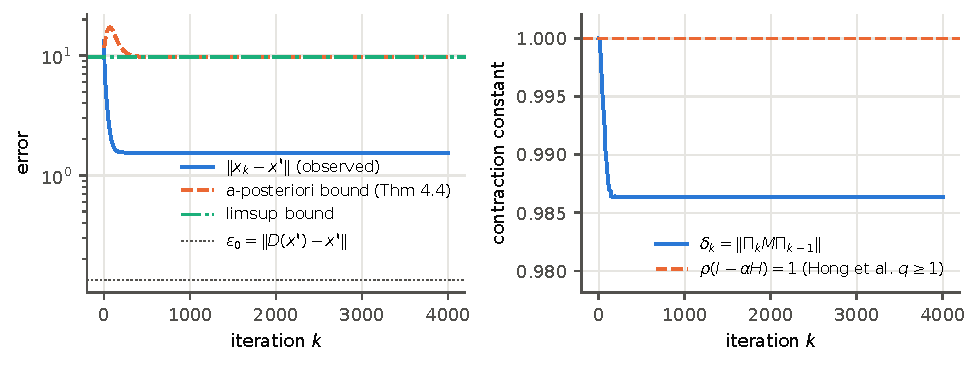
\includegraphics[width=\linewidth]{figures/ista_restricted.pdf}
\caption{PnP-ISTA with Haar soft thresholding on undersampled multi-coil data.
\emph{Left:} error to the truth, the a-posteriori bound of \cref{thm:restricted}(iv), the limsup bound
\eqref{eq:limsup} and the mismatch floor $\varepsilon_0$.
\emph{Right:} the pairwise restricted constant $\delta_k$ against the global quantity $\rho(I-\alpha H)=1$ that
governs \cite{hong2024p2np}.}
\label{fig:ista}
\end{figure}

\paragraph{The ZMSHR1 spectrum (\cref{fig:zm}).} P$^2$nP-D with the published parameters:
\begin{itemize}
\item \textbf{Safeguard.} It fired \EXPfired{} times. The smallest $\cos\angle(u_k,v_k)$ was $\EXPmincos$, against the
  guaranteed $5\cdot10^{-5}$ (\cref{cor:inert}) and $\dsg=10^{-8}$.
\item \textbf{Mixing.} It chose $a>0$ in \EXPapos{} iterations.
\item \textbf{Largest eigenvalue.} $\max_k\lmax(P_k)=\EXPmaxlam$, against the $\dsg$-free bound $10^6$ and the
  published bound $5\cdot10^{13}$. It stayed below the restricted bound of \cref{prop:restrictedzm}, with
  $U_k=$ span of the supports of $x_k$ and $x_{k-1}$, at every iteration (largest ratio $\EXPratio$). That bound is
  vacuous only in the first iterations, when $U_k$ exceeds the rank of $H$.
\item \textbf{The iteration does not settle.} The error of P$^2$nP-D drops below the PnP-ISTA limit within about
  $100$ iterations, but keeps fluctuating ($\EXPzmfinal$ at the last iteration) instead of converging to a fixed
  point. $P_k$ keeps changing with the secant direction.
\end{itemize}

\begin{figure}[t]
\centering
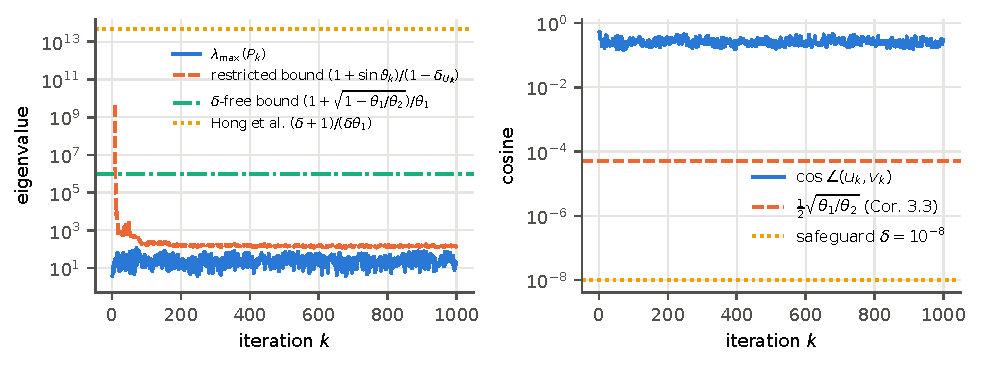
\includegraphics[width=\linewidth]{figures/zmshr1_spectrum.pdf}
\caption{ZMSHR1 along a P$^2$nP-D run.
\emph{Left:} $\lmax(P_k)$ against the restricted bound of \cref{prop:restrictedzm}, the $\dsg$-free bound of
\cref{cor:bounds} and the bound of \cite[Lemma~1]{hong2024p2np}.
\emph{Right:} $\cos\angle(u_k,v_k)$ against the lower bound of \cref{cor:inert} and the safeguard threshold.}
\label{fig:zm}
\end{figure}

\paragraph{$\theta_1$ (\cref{fig:theta}, \cref{tab:theta}).}
\begin{itemize}
\item \textbf{Small $\theta_1$ never binds.} For $\theta_1\leq10^{-2}$ the mixing step never fires: the
  restricted curvature $\inner s{Hs}/\norm s^2$ of the secants stays above $\theta_1$, as \cref{prop:restrictedzm}
  predicts.
\item \textbf{Moderate $\theta_1$ is harmless, large $\theta_1$ is not.} At $\theta_1=0.1$ the mixing step fires in about a
  third of the iterations. It damps the fluctuations of the dynamic iteration, and the late error was the lowest
  of the sweep. Once $\theta_1$ exceeds the typical restricted curvature ($0.3$, $0.6$), $a>0$ in most iterations,
  $P_k$ shrinks towards a scaled identity, and the late error grows towards that of PnP-ISTA ($\EXPthetaIlate$).
  A small \emph{worst-case} bound on $P_k$, which needs a large $\theta_1$, thus costs accuracy at a fixed
  iteration count. Moderate values cost nothing, in line with \cref{prop:restrictedzm}.
\end{itemize}

\begin{table}[t]
\centering
\caption{ZMSHR1 with different $\theta_1$ ($\theta_2=200$, $\dsg=10^{-8}$). Median error to the truth over the last
$20\,\%$ of the iterations, fraction of iterations with $a>0$, and median $\lmax(P_k)$.}
\label{tab:theta}
\begin{tabular}{lccc}
\toprule
$\theta_1$ & median late error & $a>0$ & median $\lmax(P_k)$\\
\midrule
\EXPthetatable
\bottomrule
\end{tabular}
\end{table}

\begin{figure}[t]
\centering
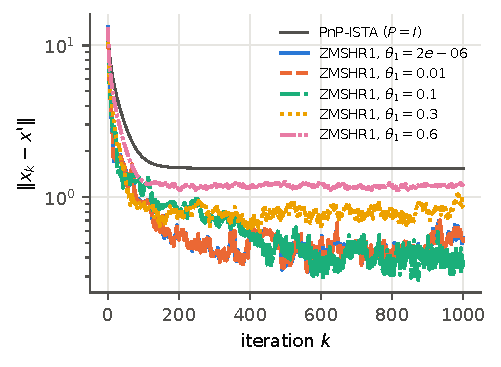
\includegraphics[width=0.55\linewidth]{figures/theta1_sweep.pdf}
\caption{Error to the truth for ZMSHR1 with different $\theta_1$ ($\theta_2=200$, $\dsg=10^{-8}$) and for
PnP-ISTA.}
\label{fig:theta}
\end{figure}

\paragraph{The estimator depends on $P$ (\cref{tab:propG}).}
\begin{itemize}
\item \textbf{Exact local model.} We take $T_0$ to be the truth's tangent space ($d_0=\EXPdG$) and the local affine
  model of soft thresholding at $\xt$. The covariances and biases of \cref{prop:estimator} are then computed
  exactly.
\item \textbf{Variance.} The tangent-restricted preconditioner reproduces the BLUE to rounding. The circulant and
  frozen-ZMSHR1 preconditioners have excess variance.
\item \textbf{Bias.} The in-tangent shrinkage bias dominates the error. $P=I$ amplifies it by up to
  $\kappa_{T_0}$. $P_T$ does not, and has both the smallest bias and the BLUE variance.
\item \textbf{Nonlinear Monte Carlo.} Over \EXPR{} noise draws we run the actual soft-threshold PnP: with $P=I$
  and with the circulant preconditioner until the relative step is below $10^{-9}$, and dynamic ZMSHR1 for a fixed
  number of iterations (it does not converge; see above).
\end{itemize}

\begin{table}[t]
\centering
\caption{Preconditioning changes the estimator.
\emph{Local affine model} (\cref{prop:estimator}): trace of the noise covariance relative to the BLUE, spectral
radius of $I-G_P$ on $T_0$ (the PnP iteration converges iff it is $<1$), and squared bias.
\emph{Soft-threshold PnP:} Monte Carlo over noise. The ZMSHR1 row uses the final $P_k$ of a P$^2$nP-D run, frozen,
in the local model, and the dynamic iteration in the Monte Carlo.}
\label{tab:propG}
\small\setlength{\tabcolsep}{4pt}
\begin{tabular}{lcccccc}
\toprule
& \multicolumn{3}{c}{local affine model} & \multicolumn{3}{c}{soft-threshold PnP (Monte Carlo)} \\
\cmidrule(lr){2-4}\cmidrule(lr){5-7}
$P$ & $\tr\mathrm{Cov}/\tr\mathrm{Cov}_{\rm BLUE}$ & $\rho(I-G_P)$ & bias$^2$ & MSE & bias$^2$ & variance\\
\midrule
\EXPpropGtable
\bottomrule
\end{tabular}
\end{table}

\paragraph{Sample complexity (\cref{fig:thmL}).}
\begin{itemize}
\item \textbf{Setup.} We fix a tangent space, draw $N_b$ shots repeatedly from $\nu$, and record how often the
  lower Chernoff event of \cref{thm:local}(a) holds ($t=1/2$). Two kinds of tangent space:
  \begin{itemize}
  \item spans of $d$ random images ($d\in\{\EXPdrand\}$), which are incoherent: $\kappa_{\rm coh}=\EXPkcohrand$;
  \item Haar tangent spaces of the phantom, i.e.\ its largest coefficients plus the coarse band
    ($d\in\{\EXPdhaar\}$), with $\kappa_{\rm coh}=\EXPkcohhaar$.
  \end{itemize}
\item \textbf{Incoherent case.} The empirical $90\,\%$ point scales linearly in $(\Phi_0/\lambda_-)\log(d/p)$, as
  \eqref{eq:Nb} predicts. The theorem's constant is conservative by a factor of \EXPconsrand.
\item \textbf{Haar case.} The points lie far below the prediction (a factor \EXPconshaar): the coherence barrier of
  \cref{rem:coherence}. $\Phi_0$ is attained at the centre of $k$-space, which variable-density sampling covers
  almost surely anyway.
\end{itemize}

\begin{figure}[t]
\centering
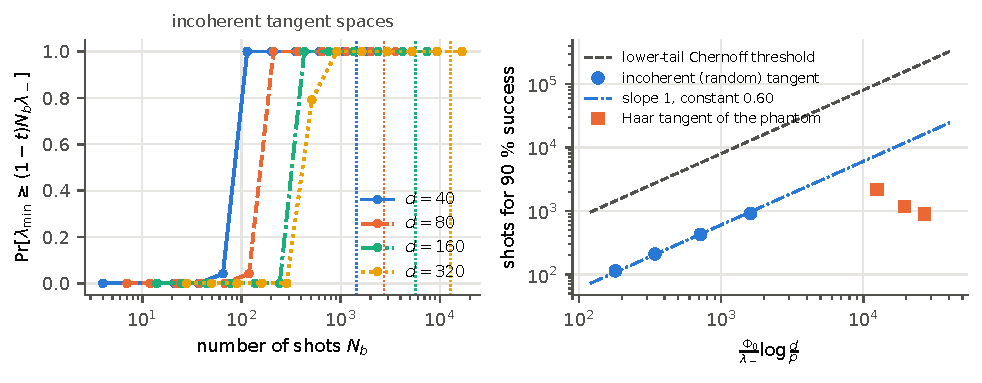
\includegraphics[width=\linewidth]{figures/thmL_chernoff.pdf}
\caption{Restricted Chernoff event of \cref{thm:local}(a).
\emph{Left:} probability versus the number of shots for incoherent tangent spaces; dotted lines mark the
lower-tail threshold $\frac{2\Phi_0}{t^2\lambda_-}\log\frac dp$.
\emph{Right:} shots needed for $90\,\%$ success against $(\Phi_0/\lambda_-)\log(d/p)$, for incoherent (circles) and
Haar (squares) tangent spaces.}
\label{fig:thmL}
\end{figure}

\paragraph{MRI-scale measurements.} \todo{4D flow pipeline, phantom ph0001, one frame, trained denoiser:
\begin{itemize}
\item $d=\tr J_D$ by Hutchinson / SURE divergence \cite{hutchinson1989,stein1981};
\item $\Pi_0$ and $\eta_0$ by block Lanczos on $\tfrac12(J+J^*)$;
\item $\kappa_{T_0}$ and $\Phi_0$ per interleaf;
\item $L_J$ by finite differences;
\item $\varepsilon_0$, and the local rate against the observed rate;
\item the excess variance of the circulant preconditioner (\cref{prop:estimator}).
\end{itemize}
Predictions to test, as in \cref{rem:local,rem:reading}:
\begin{itemize}
\item the error floor rises once total samples fall below $\sim\kappa_{\rm coh}d\log d$;
\item preconditioning lowers the error at a fixed iteration count only while the leakage condition fails without
  it;
\item the circulant limit is noisier than the $P=I$ limit;
\item $P_T$ reaches the $P=I$ limit in a few iterations.
\end{itemize}}

\section{Discussion and limitations}\label{sec:discussion}

\begin{itemize}
\item \textbf{The denoiser hypothesis.} \Cref{ass:secant} (or \cref{ass:D1}) is a hypothesis about the trained
  denoiser. Approximate symmetry and projection-like spectra of denoiser Jacobians are well documented
  \cite{mohan2020,kadkhodaie2024,manor2024}, but no theorem says that training produces small leakage. Leakage
  and Jacobian Lipschitzness can be measured with Jacobian-vector products, but only on samples, which gives
  lower bounds on suprema.
\item \textbf{Global phase.} \Cref{thm:local} covers the final, accuracy-determining phase. Convergence from a cold
  start (the analogue of support identification) is open. \Cref{thm:uniform} reduces it to a deterministic
  statement about secants along long segments.
\item \textbf{Momentum.} Accelerated variants break the one-step tangent structure ($e_k$ is no longer the image
  of a single tangent map). A three-term version of \cref{thm:restricted} seems feasible. The degradation of
  accelerated PnP reported in \cite{hong2024p2np} is a reason to do it.
\item \textbf{Prior mismatch.} Mismatch enters only through $\varepsilon_0$ and $\mu$. Distributional shift
  (phantom to patient) is not covered.
\item \textbf{Hallucination.} The trade-off between passing the truth's tangent directions ($\varepsilon_0$ small)
  and suppressing null-space directions ($\eta$ small) is a linearised form of the accuracy--stability
  trade-off of \cite{gottschling2025}.
\end{itemize}

\appendix
\section{Proof of \texorpdfstring{\cref{thm:uniform}}{Theorem 5.3}}\label{app:uniform}

\textbf{Step 1: one pair.} Fix $T,T'\in\T$ and let $Y_j=\alpha\Pi_TB_j^*B_j\Pi_{T'}$, viewed as a $d\times d$ matrix
from $T'$ to $T$, and $Z_j=Y_j-\EE Y_j$.
\begin{itemize}
\item \textbf{Uniform bound.} $\norm{Y_j}\leq\alpha\norm{B_j\Pi_T}\norm{B_j\Pi_{T'}}\leq\alpha\Phi_\T$, so
  $\norm{Z_j}\leq2\alpha\Phi_\T$.
\item \textbf{Variance.} We have
  \[
  \EE Z_jZ_j^*\preceq\EE Y_jY_j^*\preceq\alpha^2\Phi_\T\,\EE\,\Pi_TB_j^*B_j\Pi_T,
  \]
  so the variance proxy is at most $\alpha^2N_b\Phi_\T\lambda_+(\T)$. The same holds for $Z_j^*Z_j$.
\item \textbf{Tail bound.} The rectangular matrix Bernstein inequality \cite[Thm.~1.6]{tropp2012} gives, for
  $\tau>0$,
  \[
  \Pr\Big[\big\|\textstyle\sum_jZ_j\big\|\geq\tau\Big]\leq2d\exp\Big(-\frac{\tau^2/2}{\alpha^2N_b\Phi_\T\lambda_++2\alpha\Phi_\T\tau/3}\Big)
  =2d\exp\Big(-\frac{N_b\tau^2}{2a\Phi_\T(a\lambda_++2\tau/3)}\Big).
  \]
\end{itemize}

\textbf{Step 2: from a net to the family.} Let $\Delta=\alpha(H-N_b\Hb)$. On $\{\norm{\alpha H}\leq2\}$, and since
$a\lmax(\Hb)\leq1$, we have $\norm\Delta\leq3$. Let $\mathcal N_\epsilon\subset\T$ be an $\epsilon$-net. For
$T,T'\in\T$ with nearest net points $\tilde T,\tilde T'$,
\[
\norm{\Pi_T\Delta\Pi_{T'}}\leq\norm{\Pi_{\tilde T}\Delta\Pi_{\tilde T'}}+\norm\Delta\big(\norm{\Pi_T-\Pi_{\tilde T}}+\norm{\Pi_{T'}-\Pi_{\tilde T'}}\big)\leq\max_{\mathrm{net}}+6\epsilon .
\]

\textbf{Step 3: union bound.} Take $\tau=t/2$ and $\epsilon=t/12$, and apply a union bound over the
$|\mathcal N_\epsilon|^2$ pairs. Then $\sup_{T,T'}\norm{\Pi_T\Delta\Pi_{T'}}\leq t$ except with probability
\[
2d\,\mathcal N(\T,t/12)^2\exp\big(-N_bt^2/(8a\Phi_\T(a\lambda_++t/3))\big)\leq p .
\]
Finally,
$\norm{\Pi_T(I-\alpha H)\Pi_{T'}}\leq\norm{\Pi_T(I-a\Hb)\Pi_{T'}}+\norm{\Pi_T\Delta\Pi_{T'}}$.
\qed

\bibliographystyle{plain}
\bibliography{refs}

\end{document}
